
{\rmfamily
This work was previously published in ACM SIGCHI 2017 \cite{Chang:2017:Revolt} and has been adapted for this document.
}

This chapter describe the second of the two crowd systems in this dissertation that explored ways to provide global context in sourced data exploration. Unlike Alloy that focused on providing global context to the crowdworkers who were constraint by their capacity to process large amounts of data in microtasks, this second system focused on providing global context to the requesters who typically turned to crowdsourcing for its ability to scale to large datasets that they themselves do not have the capacity to process fully.
Here I focused on another common approach of data analysis of labeling items in a dataset with predefined categories, a crucial process for generating labels for training machine learning models.
Crowdsourcing provides a scalable and efficient way to construct labeled datasets for training machine learning systems. However, creating comprehensive label guidelines for crowdworkers is often prohibitive even for seemingly simple concepts. Incomplete or ambiguous label guidelines can then result in differing interpretations of concepts and inconsistent labels. Existing approaches for improving label quality, such as worker screening or detection of poor work, are ineffective for this problem and can lead to rejection of honest work and a missed opportunity to capture rich interpretations about data. We introduce \emph{Revolt}, a collaborative approach that brings ideas from expert annotation workflows to crowd-based labeling. Revolt eliminates the burden of creating detailed label guidelines by harnessing crowd disagreements to identify ambiguous concepts and create rich structures (groups of semantically related items) for post-hoc label decisions. Experiments comparing Revolt to traditional crowdsourced labeling show that Revolt produces high quality labels without requiring label guidelines in turn for an increase in monetary cost. This up front cost, however, is mitigated by Revolt's ability to produce reusable structures that can accommodate a variety of label boundaries without requiring new data to be collected. Further comparisons of Revolt's collaborative and non-collaborative variants show that collaboration reaches higher label accuracy with lower monetary cost.\cite{Chang:2017:Revolt}

%\saleema{Is it true that there is an increase?} \joseph{there is an increase in worktime. i think its fair to admit this since there is extra work (explain, categorize) in our crowd workflow. i added 'monetary' here to make it more clear.} \saleema{I'll come back to this after I go through the results section. From what I remember, one of the asynchronous variants incurred a higher cost because we required people to explain all items, not just ambiguous ones...}
%We also compare Revolt to asynchronous variants of our approach showing the benefit of real-time collaboration for reducing cost and increasing label quality. \saleema{Rephrase given async issue}\ece{Maybe rephrase the last sentence like this: Comparisons of real-time and asynchronous versions of Revolt highlight trade-offs between accuracy and cost; real-time collaboration reaching higher label accuracy in term for increased costs.}



\begin{figure}[ht]
	\centering
	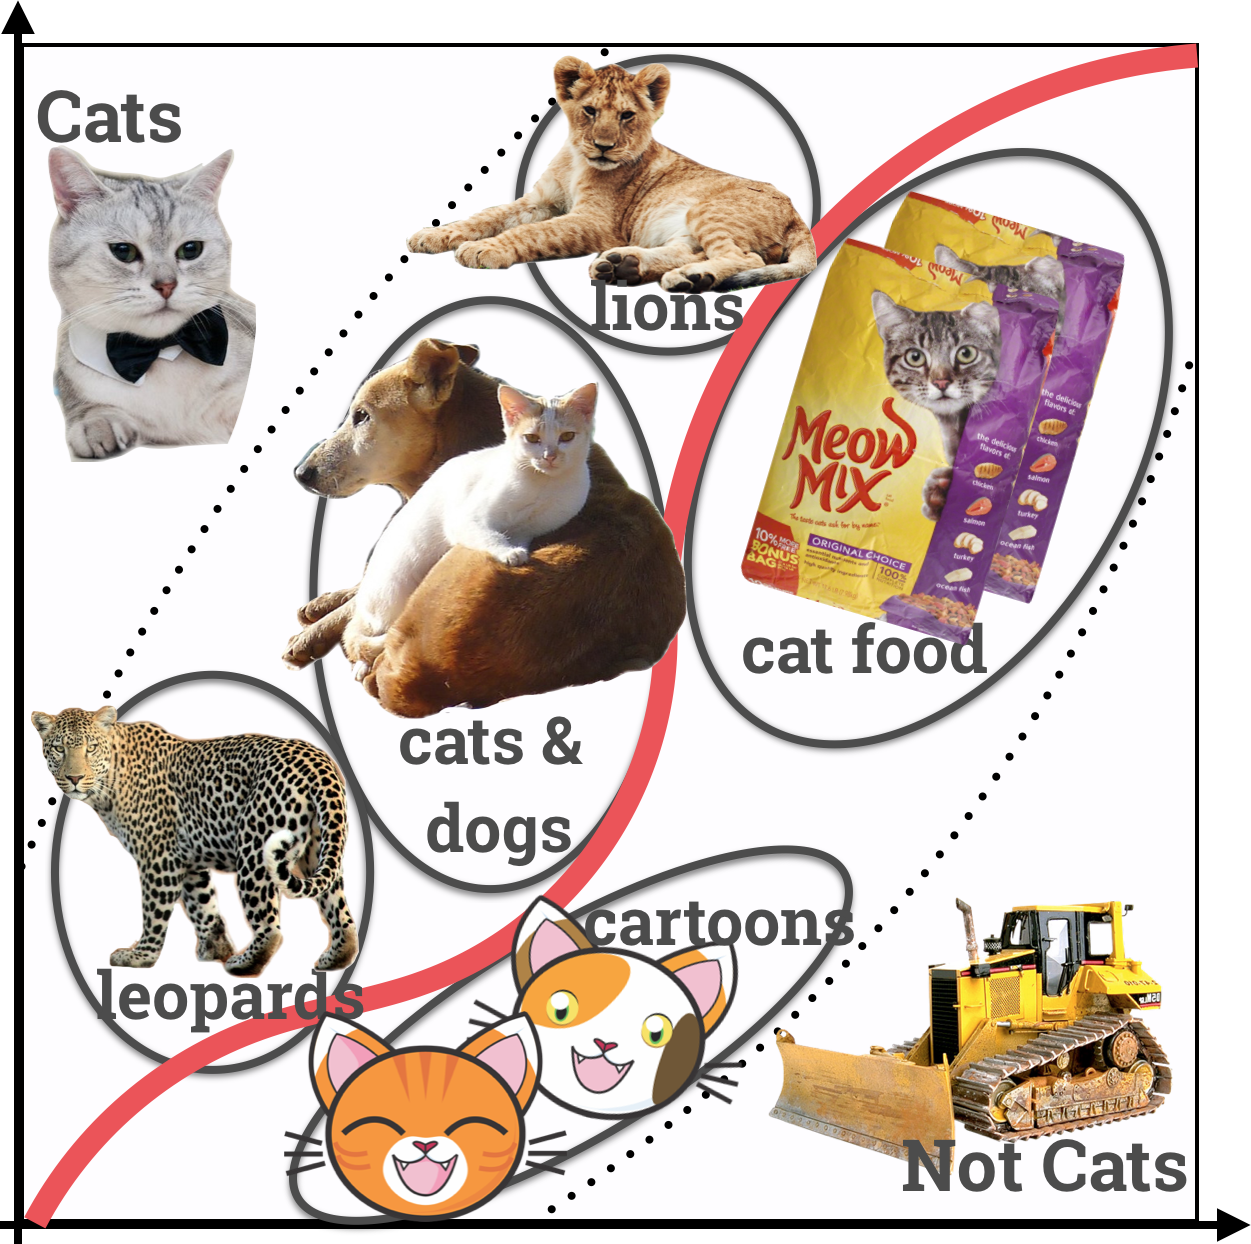
\includegraphics[width=0.45\columnwidth]{Chapters/Revolt/figures/bannerCC2.png}
	\caption[A high level view of the Revolt system.]{Revolt creates labels for unanimously labeled ``certain'' items (e.g., \emph{cats} and \emph{not cats}), and surfaces categories of ``uncertain'' items enriched with crowd feedback (e.g., \emph{cats and dogs} and \emph{cartoon cats} in the dotted middle region are annotated with crowd explanations). Rich structures allow label requesters to better understand concepts in the data and make post-hoc decisions on label boundaries (e.g., assigning \emph{cats and dogs} to the \emph{cats} label and \emph{cartoon cats} to the \emph{not cats} label) rather than providing crowd-workers with a priori label guidelines.}
	\label{fig:revolt_workflow}
\end{figure}

\section{Introduction}
From conversational assistants on mobile devices, to facial recognition on digital cameras, to document classifiers in email clients, machine learning-based systems have became ubiquitous in our daily lives. Driving these systems are machine learned models that must be trained on representative datasets labeled according to target concepts (e.g., speech labeled by their intended commands, faces labeled in images, emails labeled as spam or not spam).

Techniques for collecting labeled data include recruiting experts for manual annotation \cite{taylor2003penn}, extracting relations from readily available sources (e.g., identifying bodies of text in parallel online translations \cite{Resnik:2003:WPC:964751.964753,Chang:2012:LFT:2390665.2390698}), and automatically generating labels based on user behaviors (e.g., using dwell time to implicitly mark search result relevance \cite{agichtein2006improving}). Recently, many practitioners have also turned to crowdsourcing for creating labeled datasets at low cost \cite{Snow:2008:CFG:1613715.1613751}. Successful crowdsourced data collection typically requires practitioners to communicate their desired definition of target concepts to crowdworkers through guidelines 
explaining how instances should be labeled without leaving room for interpretation. %\saleema{Ece suggested not to use subjective in the paper. Here would be a good time to introduce the correct term, perhaps ambigous, and explain. I think the problem is in the concept definition boundary. The requester has a desired boundary that they are trying to communicate, but others may have other boundaries. Everyone can recognize a category of cartoon cats. That's not ambigious. But where you draw the boundarity is ambiguous}.  %This is redundnat so i cut it: Ideally, before enlisting the crowd, practitioners typically engage in an iterative process of generating guidelines about how crowdworkers should label items in the data. 
The guideline generation process is similar but often less rigorous than the process used by expert annotators in behavioral sciences \cite{macqueen1998codebook, weston2001analyzing} whereby experts independently examine a sample of data, generate guidelines especially around possibly ambiguous concepts discovered in the data, and then discuss and iterate over the guidelines based on feedback from others \cite{kulesza2014structured}. The guidelines are used as instructions in crowdsourced labeling tasks given to multiple crowdworkers for redundancy. Label disagreements are commonly seen as noise or failure to carefully follow the guidelines, and later corrected through simple majority voting.

%\saleema{Some redundancy between this paragraph and the last}

While traditional crowd-based labeling has produced many novel datasets used for training machine learning systems \cite{deng2009imagenet,krizhevsky2012imagenet,post2012constructing}, a common assumption in labeled data collection is that every task has one correct label which can be recovered by the consensus of the crowd \cite{bachrach2012grade}. This assumption, however, rarely holds for every item even for simple concepts (e.g., \emph{cat} vs. \emph{not cat} as illustrated in Figure~\ref{fig:revolt_workflow}) and even experts have been shown to vary their labels significantly on the exact same data due to their evolving interpretations of the target concept \cite{kulesza2014structured}. Specifying comprehensive guidelines that cover all the nuances and subtleties in a dataset would require close examination of much of the data which is typically infeasible in the crowdsourcing settings.  Crowdworkers are then often presented with incomplete guidelines and left to make their own decisions on items open to interpretation. Not only can this lead to poor quality labels and machine learning models with low accuracy, efforts to detect poor quality work (e.g.,  \cite{ipeirotis2010quality,callison2010creating,hansen2013quality}) in these cases can actually be harmful due to rejection of honest work. More fundamentally, limiting crowdworkers to providing feedback only in terms of predefined labels, failing to capture their confusions and reasoning, presents a lost opportunity to discover and capture rich structures in the data that the crowdworkers had encountered. %\saleema{This is unclear. You also say this again two paragraphs from now (and better) so I'd cut this: Aiming at discovering the structure of the data rather than only labeling it can allow for reusability of the dataset when the definitions of the target concepts evolve for the requesters or varies across different users of the dataset.} 

In this chapter, we present \emph{Revolt}, a collaborative crowdsourcing system that applies ideas from expert annotation workflows to crowdsourcing (e.g., supporting flagging of ambiguous items and discussion) for creating high quality training labels for machine learning.  Revolt enables groups of workers to collaboratively label data through three stages: \textit{Vote} (where crowdworkers label as in traditional labeling), \textit{Explain} (where crowdworkers provide justifications for their labels on conflicting items), and \textit{Categorize} (where crowdworkers review explanations from others and then tag conflicting items with terms describing the newly discovered concepts). The rich information gathered from the process can then be presented to requesters at various levels of granularity for post-hoc judgments to define the final label decision boundaries.  

Revolt requires no pre-defined label guidelines aside from the top-level concept of interest (e.g., faces, spam). As a result, this approach reverses the traditional crowdsourced labeling approach by shifting label requester efforts from guideline creation to post-hoc analysis. The rich structures provided by our approach has the additional benefit of enabling label requesters to experiment with different label decision boundaries without having to re-run label generation with the wide variety of possible label guidelines. For example, for collecting labels of images of \emph{Cats} (Figure~\ref{fig:revolt_workflow}), Revolt produces structures that group together ambiguous sub-concepts such as \emph{cartoon cats}, \emph{cat food}, \emph{leopards} and \emph{lions} along with descriptive explanations about the structures. Requesters can then review these structures and experiment with machine learning models that are trained to identify \emph{leopards} and \emph{lions} as \emph{Cats} or not. 

%\saleema{Somewhere in the paper we need to explain that here we're investigating whether Revolt produces results that contain rich enough information such that requesters could make decisions. That is, this is a necesary step in determining if our real-time collaborative aproach could be used by label requesters. We don't build a UI for label requesters to generate final labels. I'm worried about hwere this should go and how it should be carefully phrased. }

This chapter makes the following contributions:
\begin{itemize}  
\setlength\itemsep{-0.26em}
%\item A new formulation of crowdsourcing labeled data collection problem that defines the problem as a collaboration between crowds and requesters, eliminating dependency to comprehensive guidelines. \saleema{I don't think this is a contribution on its own. Are you the first to do this? I thought you mentioned in related work that there has been communication with requesters and crowds for other tasks. I'd merge this with the Revolt contribution.}   
\item A new approach to crowdsourcing label collection that employs crowds to identify uncertain aspects of the data and generate rich structures for post-hoc requester judgments, instead of trying to clearly define target concepts beforehand with comprehensive guidelines.
\item \emph{Revolt}, an implementation of our collaborative crowdsourcing approach that builds structures containing rich enough information for generating training labels for machine learning. We present both real-time and asynchronous versions of our approach. % k \saleema{Joseph, I changed this a bit to explain the real-time and async versions. Maybe adda bit to the last sentence to explain why or our main finding, that both achieve good accuracy but vary in cost.}
\item An experiment comparing Revolt to traditional crowd-based labeling on a variety of labeling tasks showing Revolt can produce high quality labels without the need for guidelines. 
\item An experiment comparing Revolt to its non-collaborative variants showing the benefits of collaboration for reducing cost and increasing quality.
%\saleema{this contradicts the abstract that says collaboration increases cost}. \joseph{the abstract is comparing Revolt to the baselines, and this is comparing Revolt to its non-collaborative variants (Solo and SoloClusterAll)}\saleema{Am I missing something? The sentence in question from the abstract is: Comparisons of real-time and asynchronous variants of \emph{Revolt} show that real-time collaboration reaches higher label accuracy in turn for an increase in monetary cost.}

%\item Findings from an informal follow up study applying Revolt to a real labeling task and presenting the resulting rich structures to a label requester for feedback. \saleema{I'm not sure we should state this as a contribution}
\end{itemize}

\section{Related Work}

\subsection{Data Labeling Techniques}

Data labeling or annotation is a common practice for many research areas. In social and behavioral sciences, researchers annotate (or code) data to build up theories about collected data, and then analyze the annotated results to discover interesting phenomena \cite{strauss1998basics}. This approach often involves multiple experts working in iterative and collaborative workflows. For example, annotators typically first examine and manually label a dataset (or subset of the dataset) independently and then compare and discuss their labels to iteratively refine a set of combined label guidelines \cite{macqueen1998codebook, weston2001analyzing}. Multiple iterations of data examination, label discussion, and guideline refinement may also occur to ensure the quality and coverage of the final guidelines. Once the guidelines stabilize, annotators can then independently label additional data accordingly to produce consistent final labels with high agreement.

Similar collaborative and iterative workflows have been reported for creating high-quality labeled datasets used in natural language processing and machine learning (e.g., \cite{marcus1993building, wiebe1999development, kulesza2014structured}). For example, Kulesza et al. \cite{kulesza2014structured} found that annotators often evolved their conceptual definition of a target concept and their corresponding labels throughout the course of observing more items in a dataset. Here, allowing annotators to create explicit structures designating ambiguous items discovered during labeling enabled them to gradually build up a better global understanding of the data and generate more consistent final labels. Wiebe et al. \cite{wiebe1999development} also proposed an iterative and collaborative workflow that relies on comparing and discussing conflicting labels amongst expert annotators to construct and refine shared labeling guidelines for producing training labels for complex datasets. 
These iterative and collaborative processes provide expert annotators systematic ways to learn about and discuss different interpretations of data during labeling. %\saleema{Joseph, which of the references in this paragraph take a collaborative approach? I think you should expand on one of them in a sentence or two. Otherwise this paragraph is just about iteration.}

While expert annotation has been used in creating labeled datasets for machine learning, this process is often too costly and time consuming to scale to the large datasets required for modern machine learning algorithms. As an example, the Penn Treebank dataset that is commonly used in natural language processing for training part-of-speech sequence labelers and syntactic parsers, was built by teams of linguists over the course of eight years \cite{taylor2003penn}. Another example from a previous work showed labeling 1,000 English sentences took four experts nine hours each to iteratively refine their guidelines by labeling items independently then discussing together \cite{wiebe1999development}. %\saleema{This wasn't a "labeling experiment" was it? I assume it was some machine learning problem that required some labeled data. Maybe something about evaluating some new algorithm with labeled data?} \joseph{the core contribution of the paper is an expert annotation workflow and a redundant label aggregation method that can produce high quality training label for machine learning models}
Many researchers and practitioners have therefore recently turned to crowdsourcing to label data for its scalability and relatively low cost \cite{deng2009imagenet,krizhevsky2012imagenet,post2012constructing}. However, despite its efficiency, researchers have also reported difficulty obtaining high quality labels using crowdsourcing \cite{alonso2013some,Demartini:2012:ZLP:2187836.2187900}. Multiple factors can contribute to poor quality labels, such as poor work from inattentive labelers, uncertainty in the task itself (resulting from poorly written guidelines or confusing interfaces), varying worker backgrounds and prior knowledge, or items that are difficult to understand by novice workers \cite{knowlton1966definition}. 

\subsection{Improving the Quality of Crowdsourced Labels}
While disagreements between expert annotators are typically resolved through discussing and refining guidelines \cite{marcus1993building}, disagreements in crowdsourcing are commonly seen as labeling errors to be corrected through majority voting over independent redundant judgments of crowdworkers \cite{kairam2016parting}. 
Methods for further improving the quality of crowdsourced labels can be mainly broken down into two camps \cite{kittur2013future}: techniques for preventing poor quality work and techniques for post-hoc detection of poor quality work. Prevention techniques include screening for crowdworkers capable of different tasks \cite{Difallah:2013:PTM:2488388.2488421,kamar2012combining}, pre-training crowdworkers \cite{doroudi2016toward}, maintaining quality while controlling for cost via dynamic task allocation \cite{Tran-Thanh:2014:BBL:2615731.2615809,bragg2013crowdsourcing}, or designing interfaces or payment structures to motivate good work \cite{mitra2015comparing,rogstadius2011assessment,hansen2013quality}. Post-hoc identification techniques include probabilistic modeling based on crowdworker agreements for weighted voting \cite{ipeirotis2010quality}, analyzing crowdworker behaviors during tasks \cite{rzeszotarski2012crowdscape}, and using additional crowdworkers to review the work of others \cite{callison2010creating,hansen2013quality}.

A common assumption in previous work is that every item has one correct label, and conflicts among crowdworkers are the result of poor quality work from novice or inattentive workers. However, constructing comprehensive and clear instructions about how to correctly label a dataset is often not possible due to the large variety of nuances and subtleties that may exist in the data, even for seemingly simple topics. For example, requesters wanting to identify \emph{cat} photos in a dataset might not be aware that the dataset also contains photos of \emph{leopards}, and/or that leopards are sometimes referred to as \emph{big cats}. As a result, crowdworkers often have to label with incomplete information. Concepts not specified in guidelines are then open to interpretation and confusion amongst crowdworkers (e.g., ``should \emph{leopards}, \emph{lion cubs}, or \emph{cartoon cats} be labeled as \emph{cats}?'' Figure~\ref{fig:revolt_workflow}), potentially leading to inconsistent labels (e.g., only some \emph{leopard} items being labeled as \emph{cats}). Methods for identifying poor work are ineffective in these cases and can be harmful to both crowdworker and requester reputations due to rejection of honest work. More fundamentally, this suggests a lost opportunity for requesters to discover interesting new concepts already identified by human computation during the labeling process since the crowdworkers are typically constrained to provide feedback in the form of predefined labels (e.g., \emph{cats} or \emph{not cats}, but not \emph{leopards}).

Even if requesters attempt to create comprehensive guidelines, they often have to review large portions of a dataset to do so which can be prohibitively expensive. Moreover, as guidelines become more complete, they can also become longer and more complicated (e.g., \cite{google} and \cite{bing}), requiring more crowdworker training or resulting in more errors. If the resulting label quality is inadequate, requesters will typically have to go through the tedious process of reviewing inconsistencies, identifying sources of confusion, updating the guidelines, and collecting entirely new labels given the updated guidelines \cite{kulesza2014structured}, potentially doubling the monetary cost of the process. 

\subsection{Harnessing the Diversity of Crowdsourcing}
Instead of treating crowdworker disagreement as noise introduced by poor work or lack of expertise, researchers have recently begun exploring methods to harness these disagreements as valuable signals. For example, researchers have found that disagreements amongst novice workers in syntactic labeling tasks often mirror disagreements amongst linguists \cite{plank2014linguistically} and are useful signals for identifying poor task designs \cite{inel2014crowdtruth}. %\saleema{Joseph, I took a pass at fixing the last bit of this paragraph. Check that it makes sense. If I'm missing something about related work, the old text is commented out below}
In another example, Kairam and Heer \cite{kairam2016parting} used label agreements to cluster crowdworkers into worker types (e.g., \emph{liberal} and \emph{conservative} labelers that identified different amount of targets in an entity extraction task). Manual analysis of these clusters were then used to improve future task designs. In contrast to this previous work, we use crowd disagreements to identify and explain ambiguous concepts in data for the purpose generating labeled data for machine learning. 

%In another example, Kairam and Heer \cite{kairam2016parting} clustered crowdworkers based on their label agreements, and manually analyzed the clusters to improve task designs through iteration. In their evaluations, clusters of crowdworkers in a named entity identification and classification task showed different characteristics, such as \emph{liberal} and \emph{conservative} workers, and also crowdworkers who interpreted the target concepts differently and labeled \emph{Botanic Gardens} as either \emph{facilities} or \emph{locations}. \saleema{Need a sentence about how our work is different from these. e.g., we use disagreements/diversity to identify and describe ambiguous concepts}

%\saleema{Joseph I revised the following paragraph. Check that it is accurate since I'm not familiar with MicroTalk}
Most closely related to our work is the MicroTalk system \cite{drapeau2016microtalk} which used crowd diversity to collect and present counterarguments to crowdworkers during labeling to improve label quality. However, this approach still assumes that a single correct label exists for every item and requires crowdworkers to pass a training stage to learn label guidelines before participating. In our work, we tackle the problem of labeling with untrained crowdworkers under the assumption that a single correct label might not exist for every item. Diversity in interpretation is then used to create rich structures of uncertain items for post-hoc label decisions, avoiding the burden of creating comprehensive guidelines beforehand and pre-training crowdworkers. We compare our approach to a condition inspired by MicroTalk called \emph{Revote}, showing that Revolt can produce training labels with higher accuracy under the scenario where comprehensive guidelines are not available.
%asked crowdworkers to justify their labels with short explanations, and present these arguments to future workers who labeled the same items differently. They found that some crowdworkers who failed to identify the correct label was able to reconsider their labels after seeing the counterarguments, increasing the overall labeling accuracy.
%However, the system required pre-constructed guidelines and pre-trained crowdworkers, and still assumed a single correct answer for all items.

%\ece{We need a stronger statement here to seperate our work from drapeau2016microtalk. Do they study the same problem we do, or do they still assume a single correct answer exists for each task and conflicts occur due to worker errors? If it is the second one, I'd start differentiating our work by saying that we study a different problem and do not make the assumptions they are making. }

%\saleema{I cut what was here because it was redundant}

%\ece{I found the following paragraph redundant given the intro. Only keeping the first sentence would suffice.} \joseph{i commented out the second sentence, its probably too specific here}
%In this work, rather than leverage crowdworker diversity for improving task designs to better generate single correct answers, we exploit crowdsourcing mechanisms to capture disagreements and root causes of disagreements as they occur, and allow crowdworkers to resolve these conflicts by creating rich structures through collaboration. 
%More specifically, we design workflows for generating high quality labels for training data by grouping crowdworkers into small ad-hoc teams, allowing them to exchange individual interpretations and report back information learned via categories of ambiguous items. These structures can then be presented to label requesters to make the final decisions without changing the tasks or hiring more crowdworkers (e.g., freely assign the \emph{leopard} category with the \emph{cat} or \emph{not cat} labels).



%\joseph{i did another pass}
%\saleema{This still sounds like a post-hoc analysis type of thing which still sounds similar to previous work. Maybe clarify what previous work used the disagreement driven structures for. Did they use it for ML? What about using it for ML makes it different? }

\subsection{Structuring Unlabeled Data with the Crowd}
Crowd structuring refers to tasks that make use of crowdsourcing for organizing information without predefined target concepts. For example, categorizing \cite{alloy,crowdsynth} or create taxonomies \cite{cascade} for a set of documents. In contrast, our work focuses on the task of \emph{crowd labeling} which is the task of assigning predefined target concepts to each item in a dataset. In our approach, crowdworkers perform structuring within a labeling task, and only to resolve different interpretations of the same items for post-hoc requester review. Past work in crowd structuring also typically involves multiple stages completed by different crowdworkers working independently, while we took a different approach by utilizing real-time crowdsourcing to maintain a shared global structure synchronized across groups of crowdworkers working collaboratively. 

%These past work on crowd structuring focused on the task of discovering topical categories in a set of textual data, while we focused on creating structures within a labeling task for resolving different interpretations of the same items from different crowdworkers. Comparing to previous work in crowd clustering, we took a simpler approach by maintaining a shared global structure synchronized in real-time across crowdworkers labeling different partitions of the dataset. In addition, before attempting to categorize items, crowdworkers in our system had already gained a rich understanding of the dataset by working on the same items in two previous stages. 

%Failure to do so could lead to categories that are overly abstract or overly fine-grained \cite{alloy}. Past work has taken different approaches to tackle this problem, such as presenting multiple items to each crowdworker \cite{crowdsynth}, organizing overlapping categories into ontological structures \cite{cascade}, or using a sampling and searching mechanism that allowed crowdworkers to actively explore the dataset for context \cite{alloy}. Past work typically involves a multistage pipeline where some crowdworkers first create categories based on different subsets of the dataset, and then presenting the crowd categories to other crowdworkers for aggregation and refinement.

%\ece{Explicitly say why previous work on crowd structuring is not the answer to our problems.}


\subsection{Real-time Crowdsourcing}
Real-time crowdsourcing has been employed for a variety of purposes including minimizing reaction time in crowd-powered user interfaces \cite{bigham2010vizwiz,Bernstein:2011:CTS:2047196.2047201,Burton:2012:CSF:2384916.2384941,laput2015zensors,lasecki2013chorus}, increasing the speed of data collection \cite{lasecki2014glance,Krishna:2016:EEE:2858036.2858115}, and improving data quality by incorporating expert interventions to guide novice workers \cite{chan2016improving,dow2012shepherding,kim2014ensemble}.
In our work, we use real-time crowd-based collaboration to improve the quality of labeled data without expert intervention. Workers engage in real-time collaboration to build rich structures of data that incorporate different crowdworker perspectives and can be analyzed post-hoc. Moreover, while most previous real-time systems employ multiple crowdworkers in a single shared workspace, our approach dynamically coordinates crowdworkers to move synchronously between stages of different subtasks. Within each stage, crowdworkers make independent judgments to be revealed to others in subsequent stages. In this way, our approach still benefits from common crowdsourcing mechanisms of verification through redundant independent judgments, but can also capture and utilize diverse crowd perspectives through collaboration. 


\section{System Design}

\begin{figure}[ht]
	\centering
	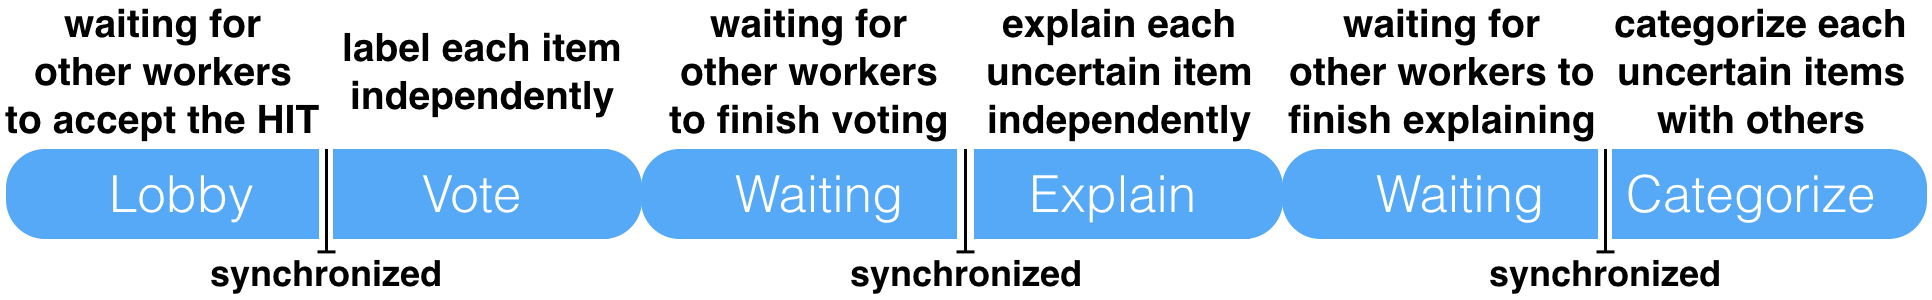
\includegraphics[width=0.9\columnwidth]{Chapters/Revolt/figures/overview3.png}
	\caption[Overview of Revolt stages.]{
	Overview of Revolt Stages: Synchronized stages requires all crowdworkers in the group to complete in order to move on. 
	}
	\label{fig:overview}
\end{figure}

In this section, we describe Revolt, a collaborative crowdsourcing system for generating labeled datasets for machine learning. Throughout this section, we use the task of labeling images as being about ``\emph{Cats}'' or ``\emph{Not Cats}'' as a running example (Figure~\ref{fig:revolt_workflow}).

At a high level, Revolt divides a dataset into multiple batches and then coordinates crowdworkers to create labels for \emph{certain} items (items receiving unanimous labels from multiple crowdworkers) in each batch and identify \emph{uncertain} items (items receiving conflicting labels) for further explanation and processing. In the synchronized version (Revolt), the system coordinates small teams of three crowdworkers through three synchronized stages: Vote, Explain, and then Categorize (see Figure~\ref{fig:overview}). In the asynchronized version (RevoltAsync), the system elicits different crowdworkers to work independently in the Vote and Explain stages, maintaining the same redundant judgement of three crowdworkers per item while eliminating the cost of coordinating crowdworkers in real-time. After collecting crowd judgments and explanations across all batches, both systems algorithmically produce structures (groups of semantically related items) at various levels of granularity for review by label requesters to determine final label decision boundaries (e.g., assigning the ``\emph{Cartoon Cats}'' category as ``\emph{Not Cats}'') before training a machine learning model. To minimize redundant information, the rest of this section describes Revolt in the context of the synchronized version. We then describe the differences of the RevoltAsync condition.


\subsection{The Vote Stage}

\begin{figure}[ht]
	\centering
	\frame{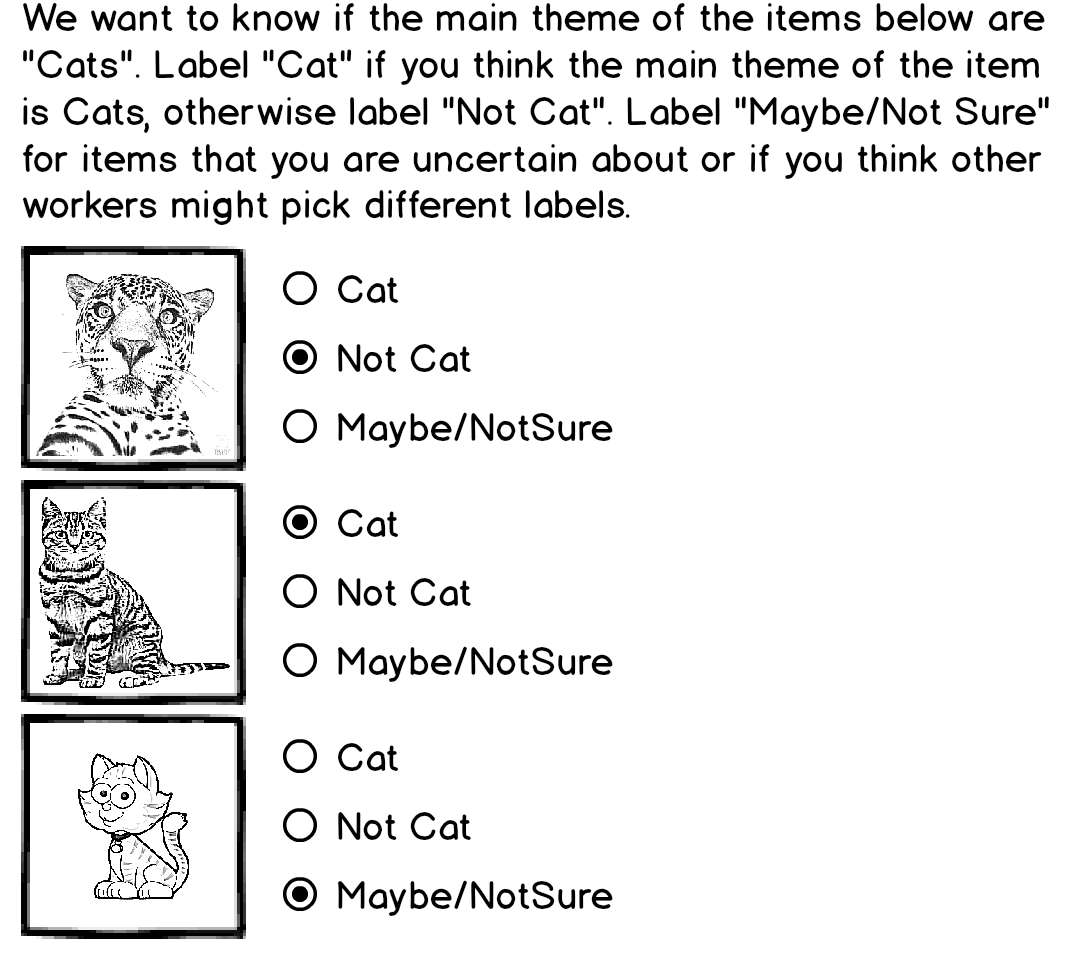
\includegraphics[width=0.6\columnwidth]{Chapters/Revolt/figures/vote.png}}
	\caption[HIT interface for the Vote Stage of Revolt]{
	Human Intelligence Task (HIT) interface for the Vote Stage. In addition to the predefined labels, crowdworkers can also select \emph{Maybe/NotSure} when they were uncertain about the item. 
	}
	\label{fig:vote}
\end{figure}

Revolt initially keeps crowdworkers in a lobby until enough crowdworkers have accepted the task and can begin as a group (Figure~\ref{fig:overview}). The Vote stage then begins by collecting independent label judgments from multiple crowdworkers using an interface similar to that used in traditional crowdsourced labeling (see Figure~\ref{fig:vote}). In addition to showing predefined labels as options at this stage (e.g., ``\emph{Cat}'' or ``\emph{Not Cat}''), we also include a ``\emph{Maybe/NotSure}'' option to ensure crowdworkers are not forced to make arbitrary decisions for uncertain items that should instead be explained further in subsequent stages. Through task instructions, crowdworkers at this stage are informed that others in the same group are also labeling the same items at the same time, and that they will be asked to compare their labels in subsequent stages. By allowing workers to express their uncertainty in the data and provide feedback in subsequent stages, Revolt avoids unfairly rejecting honest work \cite{mcinnis2016taking}.

Before Revolt can proceed to the next stage, all crowdworkers in a group must finish labeling all items in their batch. Crowdworkers who finish early are put into a waiting area where they can see in real-time how many crowdworkers in their group are still labeling items. Once the group is ready to continue, desktop and audio notifications are sent to all crowdworkers in case any stepped away while waiting. Once all labels are received, \emph{certain} items are assigned their final labels as usual, and \emph{uncertain} items (including items that received ``\emph{Maybe/NotSure}'' labels) proceed to the Explain stage.


\subsection{The Explain Stage}

\begin{figure}[ht]
	\centering
	\frame{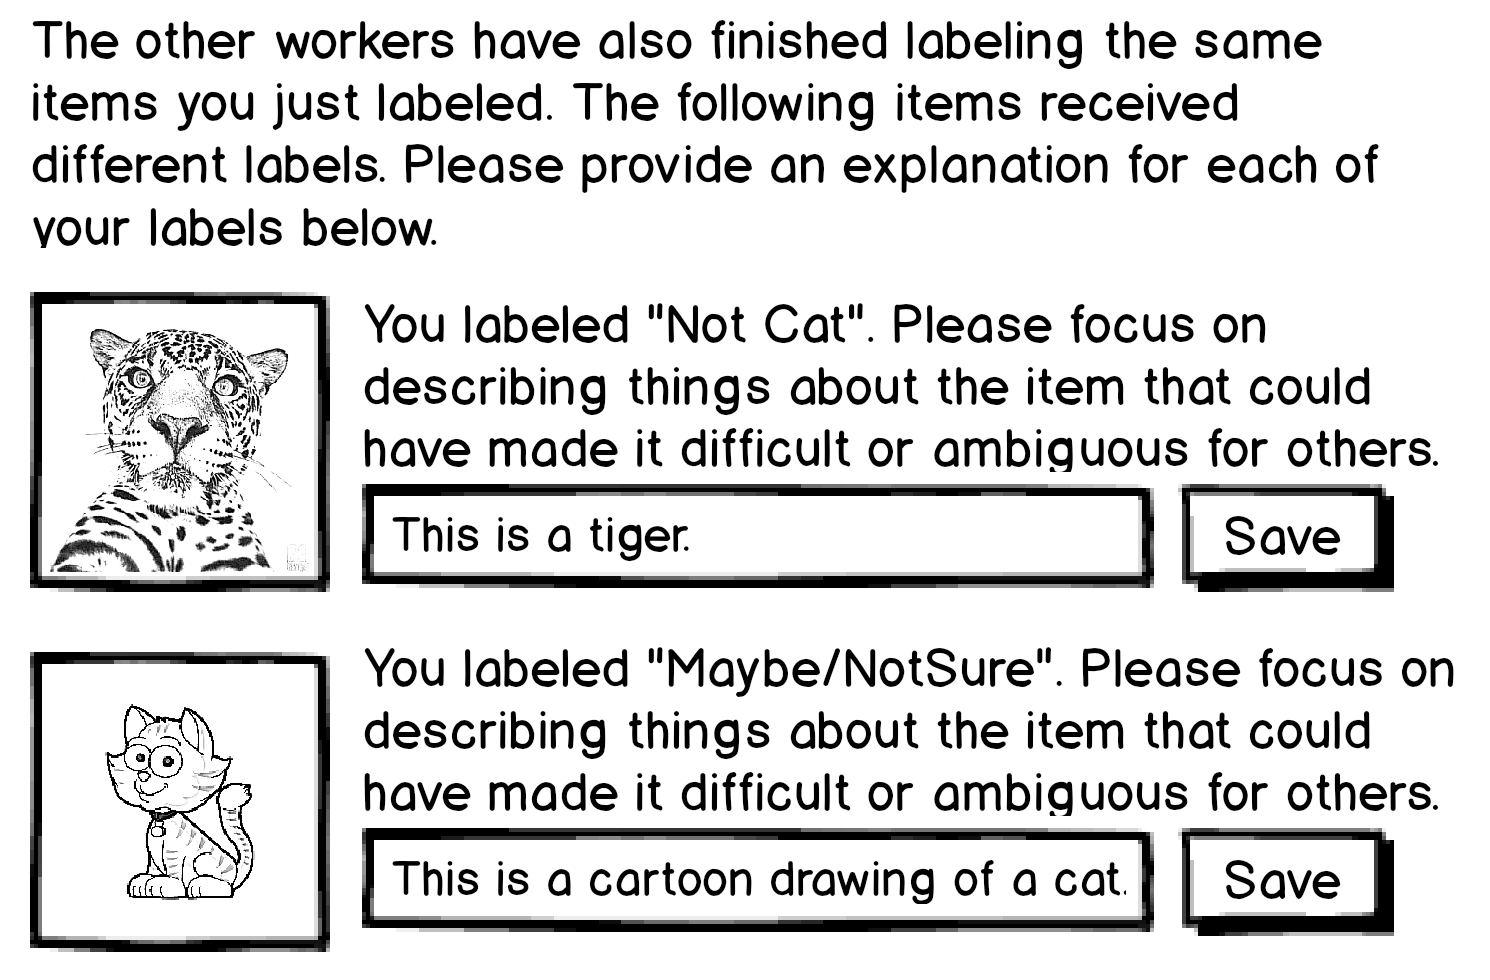
\includegraphics[width=0.6\columnwidth]{Chapters/Revolt/figures/explain.png}}
	\caption[HIT interface for the Explain Stage of Revolt]{
	Human Intelligence Task (HIT) interface for the Explain Stage. Crowdworkers enter a short description for each item that was labeled differently in the Vote Stage. They were informed that disagreement occurred, but not the distribution of different labels used. 
	}
	\label{fig:explain}
\end{figure}


In the Explain stage, crowdworkers are asked to provide short explanations about their labels for items flagged as \emph{uncertain} in the previous stage. Instructions informed each crowdworker that others in the group disagreed on the labels for these items and therefore their task was to describe their rationale for each label to the rest of the group (see Figure~\ref{fig:explain}). 

Note that early prototypes of our system also revealed the individual votes from other crowdworkers on each item at this stage. However, pilot experiments showed that this resulted in less descriptive explanations that were more focused on reacting to other crowdworkers. For example, people who picked the majority vote labels often simply reaffirmed or expressed confidence in their original label (e.g., ``\emph{nothing says to me that this is a cat}'') , whereas people who were in the minority often just yielded to the majority (e.g., ``\emph{this could be a cat, i might have messed this one up}''). Instead, hiding the labels and only stating that a disagreement had occurred resulted in more conceptual explanations helpful for the following stage (e.g., ``\emph{This is not a cat, but rather one of the big felines. Leopard or Cheetah I think.}'' and ``\emph{Although leopards are not domesticated, they are still cats.}''). As in the Vote Stage, crowdworkers who finished early were placed in a waiting area before they could move on together.


\subsection{The Categorize Stage}

\begin{figure}[ht]
	\centering
	\frame{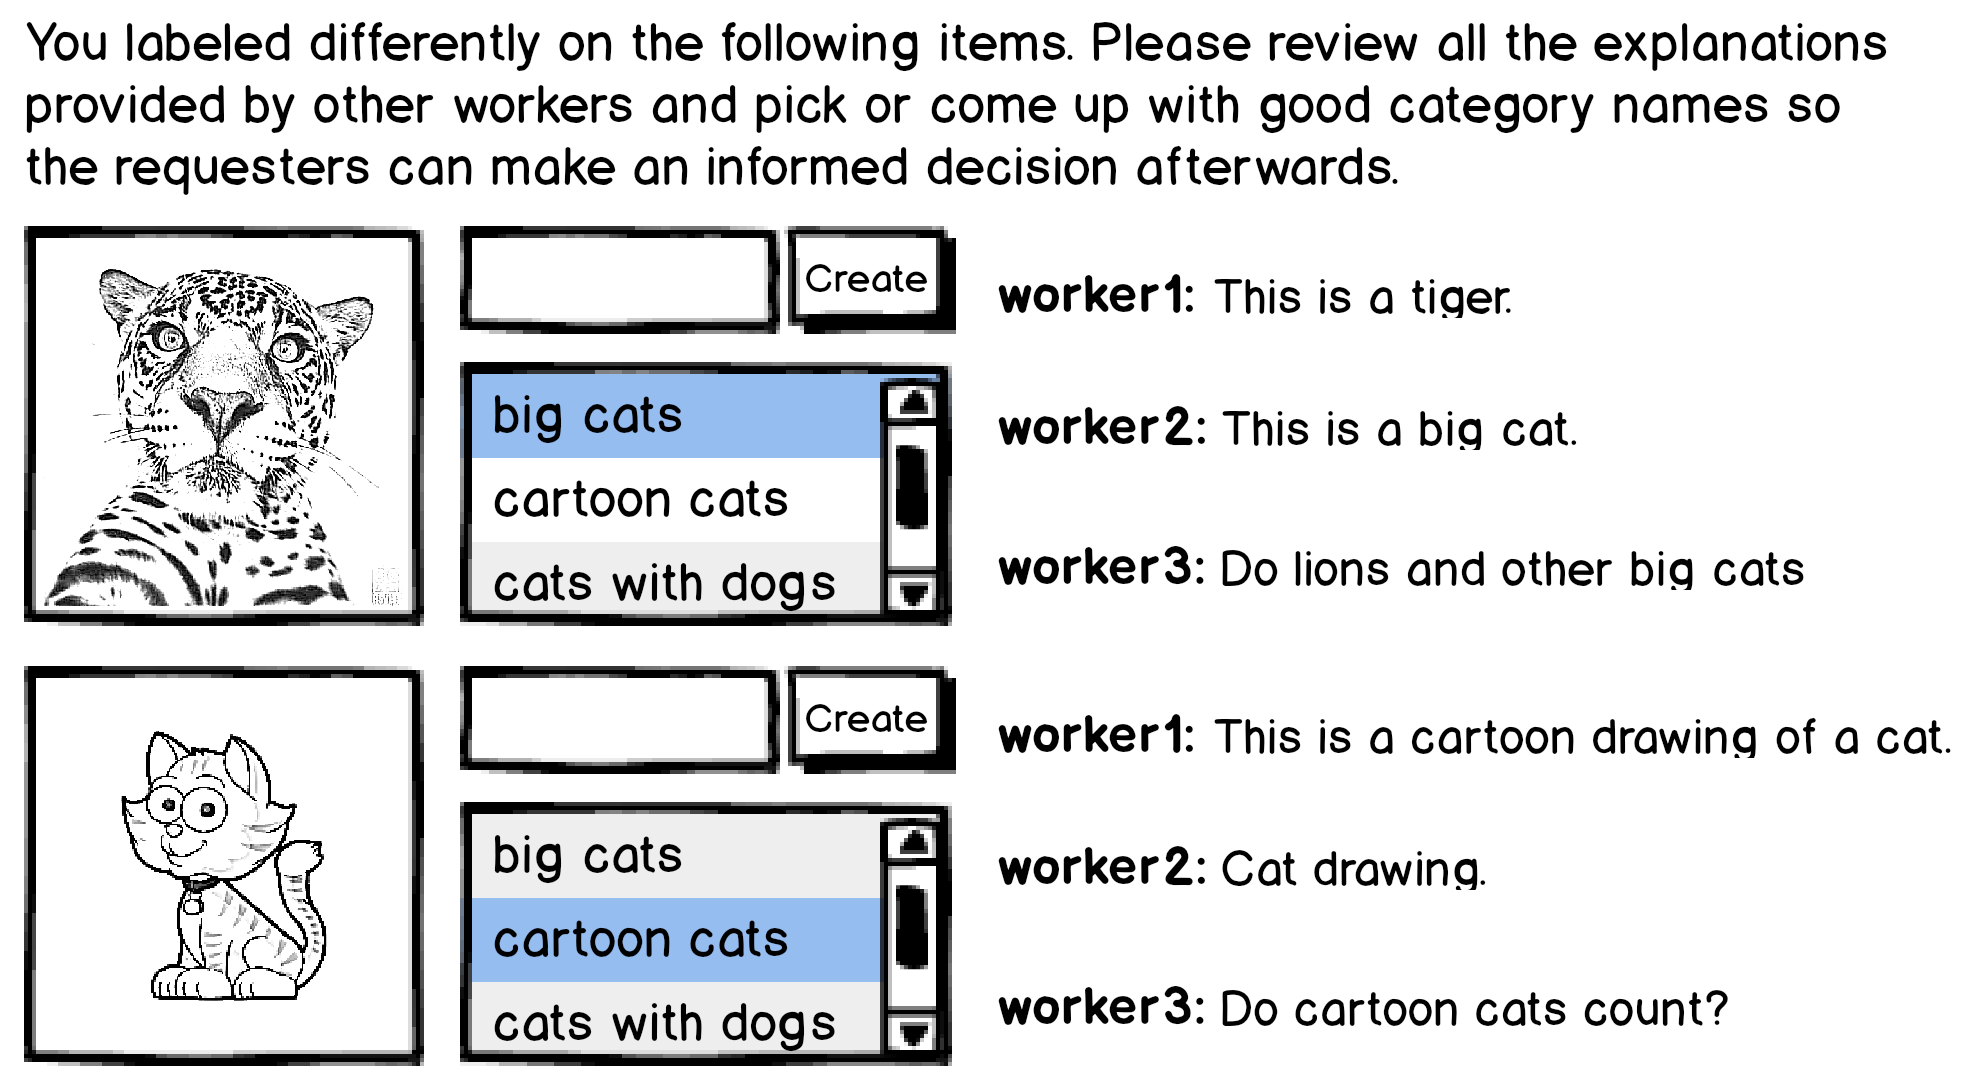
\includegraphics[width=0.6\columnwidth]{Chapters/Revolt/figures/categorize.png}}
	\caption[HIT interface for the Categorize Stage of Revolt]{
	Human Intelligence Task (HIT) interface for the Categorize Stage. Crowdworkers select or create categories for items that were labeled differently in the Vote Stage, based on explanations from all three crowdworkers in the same group. 
	}
	\label{fig:categorize}
\end{figure}


In the Categorize stage, crowdworkers were tasked with grouping uncertain items into categories based on their explanations. In this stage, we present the same uncertain items to each crowdworker again, but this time also reveal the explanations from others in the group (Figure~\ref{fig:categorize}). Crowdworkers were then instructed to categorize each item based on its explanations. Categories could either be selected from a list of existing categories presented next to each item or added manually via a text input field. Whenever a new category was added by a crowdworker, each list of categories was synchronized and dynamically updated across all items within the current group, and also across groups working on different parts of the dataset. To encourage category reuse and reduce redundancy we also implemented two mechanisms: First, the text field for creating categories also acts as a quick filter of the existing categories so that crowdworkers may more easily see and select an existing category rather than create a new one when appropriate. Second, the list of existing categories is sorted by the number of crowdworkers (across all batches of the same dataset) that have used each category, a similar strategy to that used to filter out low quality crowd categories in \cite{cascade,chilton2014frenzy}. % Here we used simple realtime crowdsourcing techniques to categorize the uncertain data, however, many more sophisticated (yet often more costly) none realtime solutions also exist in previous work. \ece{say a bit more here. How do these approaches look like? Do they depend on crowdsourcing or some automated approaches?} We will discuss the limitations of our approach in the Discussion Section. % im cutting this for space...
After assigning categories, crowdworkers could submit their HITs independently without waiting for others to complete.  
 
%\saleema{Explain the problem first. E.g., "In pilot experiments we noticed that naively updating the list or sorting the list in some way, resulted in too many redundant or synonymous categories". Then describe your solution: Two simple mechanisms were implemented to reduce redundant or synonymous categories. First, as the crowdworkers typed in the text input box for creating a new category, the category list will update and show only category names that contain the user input. Second, the list of existing category is sorted by the number of crowdworkers that have used each category, a similar strategy that was also used in past research for filtering out low quality crowd categories \cite{cascade}.}

\subsection{Post Processing of Crowdworker Responses}
%\ece{This section needs a bit more work. Here are my main issues: (1) We discuss two different ways of creating categories: simple majority voting and clustering. Which one do we do? If we do clustering at the end, why even talk about majority voting? I thought we were using majority voting categories as constraints in clustering. If so, we should say so. (2)As far as I understand, the clustering step works on explanations. if you are applying clustering at the end, how do you use the categorize stage after all? Is the categorize step unnecessary if you are using clustering? It is unclear how you are jointly using the outputs of explain and categorize steps in clustering. }
After crowdworkers in all groups have gone through all three stages, Revolt collects the crowd feedback for all batches. Revolt assigns labels to \emph{certain} items directly, and then creates structures of \emph{uncertain} items by applying simple majority voting on the category names suggested by crowdworkers for each item. In cases where all crowdworkers suggested a different category, a random crowdworker's category is used as the final category. At this point, structures can be presented to label requesters for review and to make final label decisions. For example, after reviewing structures, a label requester may decide that \emph{leopards} and \emph{lions} should be considered \emph{Cats} while \emph{cartoon cats} and \emph{cat food} should be considered \emph{Not Cats}. In this way, label assignments can be applied to the data in each category prior to training a machine learning system.


Revolt can also expand the crowd-generated categories to different numbers of clusters, supporting inspection at different levels of granularity. To do this, Revolt performs a hierarchical clustering method that uses the crowd categories as connectivity constraints. 
%\saleema{The previous sentence suggests that Revolt is an incomplete system because you say that it relies in input requesters to do the final step. You have to be very careful in how you phrase this. I'd simply say that at this point requesters can view categories to make decisions. To better support the requester, Revolt can also perform a post processing step to break down or build up categories at different levels of granularity etc...}
%Once clusters are created, the requester input is used to assign clusters to labels 
This post-processing approach works as follows:
First, a term frequency-inverse document frequency (TF-IDF) vector is used to represent each uncertain item where each dimension is the count of a term in its explanations divided by the number of uncertain items with the same term mentioned their explanations. Then, hierarchical clustering with cosine similarity is applied. That is, initially, each item is treated as a cluster by itself. Clusters are then iteratively merged with the most similar clusters, prioritizing clusters with items in the same crowd category, until all items are in the same cluster. 

Generating clusters at various levels of granularity allows label requesters to adjust the amount of effort they are willing to spend in making labeling decisions, allowing them to manage the trade-off between effort and accuracy. For example, labeling low level clusters allows for more expressive label decision boundaries, but at the cost of reviewing more clusters. 



% \saleema{This section needs work. 1) Do you need to talk about how to collect all items together from different batches distributed across different groups of workers? If so this should go here. 2) Then talk about the majority voting for categorization. Is it possible for requesters to look at these results directly, without clustering? If so, then describe how the categories can be presented to requesters for assignment. If your system relies on clustering to produce the groups that requesters should review then explain that first and give more details about the clustering than you have below}

% \saleema{Original text: For example, assigning the label \emph{cat} to all uncertain items in the category \emph{leopards}. In addition, the system also used the crowd categories as clustering constraints and run bottom-up clustering of the uncertain items using TF-IDF weighted cosine similarity of the explanations. This way the requesters can freely choose the number of categories they want to label as a trade-off between the amount of post-hoc requester efforts and the accuracy of the final labels. For example, in an extreme case, the requesters can re-label all uncertain items to gain higher labeling accuracy. In this study, we assume the requesters are capable of choosing the best label for each category that increases the accuracy of the final labels the most. We will discuss this further in the Evaluation and Discussion and Future Work Sections.}

\subsection{RevoltAsync}
RevoltAsync removes the real-time nature of Revolt as follows: One set of crowdworkers label items independently in the Vote stage. RevoltAsync then still uses the results of three crowdworkers per item to identify uncertain items. Uncertain items are then posted to the crowdsourcing market again for a different set of crowdworkers to explain the labels. That is, in RevoltAsync's Explain stage, crowdworkers are presented with an item and a label given by another crowdworker and then asked to justify that label given the knowledge that there were discrepancies between how people voted on this item.

RevoltAsync does not include a Categorize stage, which would require synchronization. Instead it uses the explanations collected at the Explain stage directly for clustering during post-processing. Clustering of explanations is still performed using hierarchical clustering, to produce structures at different levels of granularity, but without connectivity constraints based on the crowd categories provided by the Categorize Stage.



\section{Evaluation}

In this section, we describe experiments we conducted to investigate the cost-benefit trade-off of Revolt compared to the traditional crowdsourcing approach for collecting labeled training data. We also examined several variants of Revolt to better understand the benefits of different components of the Revolt system and workflow. 
%Since the design space of collaborative labeling workflows is not limited to the one described in the earlier section, we also experimented with  variants of Revolt. \saleema{Rephrase that last sentence. Saying that Revolt is just one instance of a design space minimizes the contribution. In fact you tried many different versions of Revolt we got to something that worked well. Plus this statement is true for all UIs. Just explain why you wanted to try async and other variants, e.g., to examine the benefits of real-time over...}

To compare these workflows, we ran each condition on a variety of datasets and measured the accuracy of the resulting labels with respect to requester effort and crowdsourcing cost. To prevent learning effects, we do not reuse crowdworkers across conditions for the same dataset, and randomize posting order of condition and dataset combinations so that crowdworkers subscribed to postings from our requester account using third party services\footnote{http://www.turkalert.com/} were distributed across conditions.

\subsection{Baselines and Conditions}

Our conditions include Revolt, RevoltAsync, three variants, and two baselines representing traditional labeling approaches:

\begin{itemize}
    \setlength\itemsep{-0.2em}
	\item \emph{NoGuidelines}. A baseline condition where crowdworkers label items without guidelines. This condition should be considered a lower bound baseline, since in most real world scenarios requesters are likely to have some knowledge of the data or desired labels to create some initial guidelines. 
	\item \emph{WithGuidelines}. A baseline condition where crowdworkers label items according to provided guidelines. For this condition we endeavored to create comprehensive guidelines that left no room for subjective assessment as explained in the next Datasets and Guidelines section. Since creating comprehensive guidelines is often infeasible in realistic machine learning tasks, the results from this baseline should be considered an upper bound for what can be achieved with traditional crowdsourced labeling.
	\item \emph{Revolt}. Our proposed Vote-Explain-Categorize workflow with synchronized real-time collaboration.
	\item \emph{RevoltAsync}. Our Revolt variant with asynchronous collaboration mechanisms.
	\item \emph{Revote}. A Revolt variant with similar strategies used in \cite{drapeau2016microtalk} wherein crowdworkers re-label uncertain items after considering each others' explanations instead of categorizing them for post-hoc requester review. This variant replaces Revolt's Categorize stage with a Revote stage (without the \emph{maybe} option) and uses simple majority voting to assign final labels to all items.
	\item \emph{Solo}. A Revolt variant with no collaboration. In this condition, each crowdworker labels and explains their labels for all items independently. The system still computes uncertain items from three redundant labels and clusters uncertain items using their explanations.
	\item \emph{SoloClusterAll}. A variant of \emph{Solo} where the system clusters all items based on their explanations. Note that clustering all items (certain and uncertain) is only possible in the \emph{Solo} variants where explanations were collected on all items. This approach creates categories for certain items as well as uncertain, requiring requester review of even items that reached consensus through crowd labeling.  
\end{itemize}

Note that no post-hoc requester effort is required in the NoGuidelines, WithGuidelines and Revote conditions and only the WithGuidelines baseline requires requesters to create guidelines prior to crowd labeling. We implemented the Revolt, Revote, Solo, and SoloClusterAll conditions using the TurkServer library \cite{mao12:turkserver}, which provided the infrastructure for recruiting and coordinating crowdworkers in real-time. Labels for the RevoltAsync, NoGuidelines, and WithGuidelines conditions were collected through the Mechanical Turk form builder feature on the requester interface. %\saleema{Mechanical Turks Form builder features?}


%\ece{I think this is out of place here. We never described how we use the categories to constrain the hierarchical clustering approach. Also this explanation is not enough, why we are doing this, why his helps.}
%For conditions that does not perform the realtime collaborative Categorize Stage, we use the clustering method described in the previous section to generate clusters at various granularity for post-hoc requester judgements. 
%\saleema{This is unclear. You do perform clustering on Revolt results whihc does have a Cateogrize stage. You also mention clustering in all the conditions so this is somewhat redudnent. If you want to mention clustering in the conditions, explain that you can produce clustering at various levels of granularity there.}

%\saleema{You also need a bit about how you implemented these conditions. Hee or in a new subsection on implementation. You should mention that Revolt was built over turkserver etc. Whereas the other condiitons were run over Mturk forms. This will be important when you get to cost and how you can't really compare these effectively.}


%\saleema{This section is super hard to follow and needs restructuring. Here's what I'd suggest: 1) In the intro paragraph to this section, describe the goal of our evaluation at a super high level which was to evaluate Revolt in terms of the cost benefit tradeoff compared to the traditional technique for generating labels. We also experiment with some variants of Revolt including [something about c3] and asychrnous variants to investigate the benefits of real-time collaboration. Then say, to compare these different workflows, we run each workflow on a variety of datasets and measure label accuracy and cost. 2) Put the Conditions subsection first. Make this mostly a bunch of bullet points briefly describing each of the conditionsn. 3) Put the Datasets next. 4) Then the Evaluation Metrics. This section should talk both about measuring accuracy and measuring cost. Alternatively, you can talk about how you measure accuracy in the Accuracy results section.}


%\joseph{move from results}
%In the first variant, we used the same workflow of Revolt with only one crowdworkers in each group, and increase the number of total groups so that all items are still labeled by three crowdworkers. Under this condition, crowdworkers can immediately move to further stages without waiting for other crowdworkers to finish the current stage. However, since crowdworkers are working independently, the system can not identify which items are uncertain in the Explain Stage, so the crowdworkers were asked to enter explanations for all items they have labeled. We also removed the Categorize Stage that is driven by a shared list of categories synchronized in real-time. We tested two conditions with this variants. In the Solo condition, the system identified the uncertain items after crowdworkers finished labeling and explaining all items, and create clusters of 




\subsection{Datasets and Guidelines}
% For generating each gold-standard label sets, we went through each item in the datasets in two passes, writing down notes and categories next to the items that can be open to interpretation in the first pass, and creating the final labels and write down labeling guidelines in the second pass.  These guidelines are likely to be unrealistically comprehensive comparing to guidelines used in most crowdsourcing labeling tasks, but we wanted to see how Revolt performs comparing to this upper bound condition.}

%\saleema{I took a pass at this section, but it might still be a bit confusing...}

We evaluated each of our conditions with eight tasks made up of different data types (images and webpages) and sizes (around 100 and 600 items, respectively). All of our datasets were obtained from the publicly available ImageNet \cite{deng2009imagenet} or Open Directory Project\footnote{https://www.dmoz.org/} databases, both commonly used for machine learning research. 

Each labeling task asked crowdworkers to label each item in a dataset as belonging or not belonging to a given concept. We used target concepts of \emph{Cars} and \emph{Cats} for our image datasets and \emph{Travel} and \emph{Gardening} for our webpage datasets to show that interpretations can vary for even seemingly simple and generally familiar concepts (Table~\ref{tab:accuracy}). For our \emph{Cars} and \emph{Cats} image datsets, we collected images from ImageNet \cite{deng2009imagenet} by first collecting all images that corresponded to WordNet \cite{miller1995wordnet} concepts containing the keyword ``car'' or ``cat'', and then sub-sampling the set down to approximately 600 images per dataset while ensuring no sub-concept (such as \emph{sports car} or \emph{cable car}) was overrepresented (>10\%) in the final set. We obtained our \emph{Travel} and \emph{Gardening} webpage datasets from \cite{kulesza2014structured} which has approximately 100 webpages for each concept obtained from the Open Directory Project by selecting half from each category, ``travel'' or ``gardening'', and then selecting the remainder randomly from the database.

For each dataset, we generated two sets of gold-standard labels and corresponding guidelines (making eith datasets total) representing two different interpretations of the same concept in the following way: 
%For each dataset, each author generated a set of gold-standard labels and corresponding guidelines according to their own interpretation of the target concept, acting like a label requester defining their desire label boundaries for their task.
Independently, each author first manually labeled the datasets using a structured labeling process \cite{kulesza2014structured} where they would categorize items as they examined them and then assign final labels at the end. This resulted in gold-standard labels and guidelines describing those labels (defined by rules each author would write down describing their categorizations and final label assignments) for that dataset. These guidelines can be considered comprehensive given that each item was examined during labeling. In realistic tasks with potentially large or complex datasets, it is often infeasible for label requesters to manually examine each item in order to create a set of guidelines (instead they typically examine a subset). Table~\ref{tab:accuracy} summarizes our datasets. To give some insights into the level of ambiguity that existed in each datasets, we report the proportions of items that received conflicting labels under the NoGuidelines conditions as $\mu$. The average proportion of items being assigned the positive labels in each dataset is 0.41 ($\sigma=0.12$).  
%\saleema{I took out this bit because it was confusing at this point since we haven't mentioned gold-standard labels yet...see if you can put it back somewhere that makes sense: This resulted in 39\% to 56\% of the items being assigned the positive labels in the gold-standard.} // moved from previous paragraph

%For each dataset, each author generated a set of gold-standard labels and corresponding guidelines according to their own interpretation of the target concept, acting like a label requester defining their desire label boundaries for their task.
%Independently, the authors first manually labeled the datasets using a structured labeling process \cite{kulesza2014structured} where they would categorize items as they examined them and then assign final labels at the end. This resulted in gold-standard labels and guidelines describing those labels (defined by rules each author would write down describing their categorizations and final label assignments) for that dataset. These guidelines can be considered fairly comprehensive given that each item was examined during labeling. In realistic tasks with potentially large or complex datasets, it is often infeasible for label requesters to manually examine each item in order to create a set of guidelines (instead they typically examine a subset). Table~\ref{tab:accuracy} summarizes our datasets.

%, and to give some intuition about the amount of uncertainty of each dataset, we also report the proportion of uncertain items $\mu$ that received conflicting labels when crowdworkers were labeling with the NoGuidelines condition. \saleema{What happened to Table 2? I don't see it. You should also explain why we care about the proportion of uncertain items. Are you going to do an analysis of results based on uncertainty or at least a discussion about how the proportion of uncertainty impacts things? I don't think you should get rid of this, but just be sure to disucss it later}

% \saleema{We should add this, but it might be better in the results section: . }


%For each dataset, we generated two sets of gold-standard labels (e.g., \emph{cats} or \emph{not cats}) and guidelines by labeling every item. To ensure the quality and consistency the gold-standard labels, we used a structured labeling process similar to \cite{kulesza2014structured}, examining the items in two passes, writing down notes and categories next to the items that can be interpreted differently, and creating final labels and guidelines in the second pass. 




%\subsubsection{Images from ImageNet}
%The ImageNet database consists of around 14 million images\footnote[1]{as of September of 2016} labeled with concepts from the WordNet ontology (also called \emph{synonym set} or \emph{synset} for short) \cite{deng2009imagenet}. Each of these concepts consists of a short definition and a set of synonymous phrases that refer to the concept \cite{miller1995wordnet}.
%The WordNet database consists of around 120 thousands synsets \footnote[1]{} organized in ontological structures \cite{miller1995wordnet}.
%For example, the synset \emph{\{dog, domestic dog\}} has the hypernym of \emph{\{canine, candid\}}, which in turn has the hypernym of \emph{\{carnivore\}}.
%However, this can sometimes be problematic in practice due to the ambiguity of natural language.
%For example, searching WordNet with the term "dog" leads to \emph{\{dog, domestic dog\}}, but also \emph{\{frank, hotdog, dog\}}, \emph{\{dog (informal term for a man)\}}, and five other concepts.
%To select subsets of images for labeling, we randomly selected two sets of around 600 images that correspond to WordNet synsets containing the words "cat" or "car", respectively. Since the images were already labeled, one obvious approach was to create gold-standard labels and guidelines at the synset level. However, the ImageNet dataset was also labeled by crowdworkers, and we wanted to err on the side of caution. We therefore relabeled the individual images using the approach described in the previous subsection, ans was able to correct a small number of errors.
%(For example, one photo of a house cat sitting on an image scanner was labeled with the synset \emph{\{CAT scan, CT scan\}}.)

%\subsubsection{Webpages from the Open Directory Project}

%\joseph{briefly describe the Open Directory Project, the criteria used in the structured labeling paper to select the webpages, give an example of why some webpages might be ambiguous, and point readers to the structured labeling paper for detail} 



%\saleema{I don't think this formalism is adding anything. Much of this formalism is also just talking about the workflow which you already described in the Revolt section. For example, you should have already explained in the Revolt section how you use majority voting for assigning category labels to items. So can we simplify this and just explain our technique verbally. Something like "Revolt produces labels on certain items and categorizes uncertain items into groups (you should have already explained the clustering in the Revolt section) that are intended to be reviewed by requesters to make final labeling decisions. We simulate requester assignments to categories by [describe assigning to majority class label]. Explain that this is a reasonable simulation because at the very least, without any UI support for generating group summaries or anything, you would expect that the requester could view one or two items in a category in order to make an assignment decision. Then you can say something about the likelihood of picking an item from the majority in the group. Once you've assigned each item to the positive/negative class using the direct results for certain items and the simulated category assignments you can just measure accuracy against the ground truth as normal. You should also mention here that because your system can produce groups at various levels of granularity using the bottom up clustering you described earlier, you can measure accuracy and cost at each level of granularity.}



\begin{table}[ht]
\centering
\footnotesize


\begin{tabular}{r r r r | r r r | r r r r r}

\hline
% & & & C1 & C2 & C3 & C5 & C8 & C9 & &  \\
Dataset & Type & N & $\mu$ & NoGdlns. & W/Gdlns. & Revote & Revolt & Solo & SoloAll & RVAsync & \#Cats \\
\hline
Cars1   & img & 612 & .27 & .843 & .887 & .820 & \textbf{.904} & .863 & .884 & .882 & 32 \\
Cars2   & img & 612 & .27 & .756 & .804 & .775 & \textbf{.827} & .794 & .807 & .820 & 32 \\
Cats1   & img & 572 & .12 & .844 & \textbf{.939} & .845 & .916 & .720 & .900 & .902 & 14 \\
Cats2   & img & 572 & .12 & .920 & \textbf{.962} & .904 & .935 & .787 & .916 & .918 & 14 \\
Travel1 & web & 108 & .24 & .759 & .870          & .787 & \textbf{.880} & .815 & .806 & .870 & 22\\
Travel2 & web & 108 & .24 & .769 & .870 & .759 & \textbf{.889} & .796 & .796 & .870 & 22  \\
Garden1 & web & 108 & .12 & .806 & .843 & .787 & \textbf{.889} & .861 & .759 & .852 & 8  \\
Garden2 & web & 108 & .12 & .778 & .833 & .787 & \textbf{.843} & .815 & .787 & .787 & 8  \\
\hline

\end{tabular}

\caption[Evaluation for Revolt --- Labeling accuracy under different conditions.]{Accuracy of different labeling conditions. The number of clusters of the Solo, SoloClusterAll, and RevoltAsync conditions were fixed to the number of categories observed under the Revolt condition. Bold numbers indicate the best performing condition for each dataset.}
\label{tab:accuracy}
\end{table}



%\subsection{Results}
%\saleema{From original intro:} Results suggest that when workers were labeling without guidelines, Revolt was able to produce higher labeling accuracy comparing to the traditional crowdsourcing labeling approach. Comparing against when crowdworkers were labeling with the comprehensive guidelines, Revolt was still able to produce labels with comparable accuracy, but does not require the requesters to take on the strenuous task of creating comprehensive guidelines beforehand. 
%In terms of monetary cost, Revolt does required higher crowd work-time \joseph{is this the right word?} to identify, explain, and categorize the uncertain items, but the generated rich structures also grant the requesters the ability to freely recreate and experiment with different decision boundaries at no extra monetary cost. For example, using the same output labels and categories of the uncertain items, Revolt was able to maintain good accuracy on the different gold-standards of the same datasets with minimal requester efforts of recreating the boundaries using the crowd categories, whereas the traditional approach would require the requesters to update the guidelines and hire more crowdworkers to re-label the entire dataset.  in such case

%In addition, we also tested different variants of the proposed method that does not require the crowdworkers to work collaboratively in groups, and results suggest that collaboration may be one key to Revolt's effectiveness in producing labels with good accuracy. We will discuss these findings further in the Evaluation Section.


\subsection{Results}
% For evaluation, we compute accuracy by simulating post-hoc requester judgments in the following way for all conditions. For items with final label assignments (all items in the baseline conditions, the Revote condition, and items receiving unanimous votes in the Revolt conditions) we simply use the final label directly.
 

%For uncertain items (only in Revolt or Revolt variant conditions), we assign labels to categories or clusters by taking the majority vote label as the final label for all items in the cluster \saleema{phrase that better}. 


\begin{table}[ht]
\footnotesize
\centering
\begin{tabular}{r r r l r l}
\hline
Category & Size & \multicolumn{2}{c}{Car1GdStdLabel} &\multicolumn{2}{c}{Cars2GdStdLabel} \\ 
\hline
train car           & 19    & 95\% & not car   & 95\% & not car \\
train               & 19    & 100\% & not car  & 100\% & not car \\ 
military vehicle    & 16    & 100\% & not car  & 100\% & not car \\ 
car                 & 15    & 73\% & car       & 53\% & not car \\         
vehicle mirror      & 14    & 100\% & car      & 100\% & not car \\         
bumper car          & 12    & 100\% & not car  & 100\% & not car \\ 
tow truck           & 11    & 91\% & car       & 91\% & car \\         
wheel               & 8     & 100\% & car      & 88\% & not car \\         
truck               & 8     & 100\% & car      & 75\% & car \\         
trolley             & 7     & 86\% & car       & 86\% & car \\         
vehicle interior    & 6     & 100\% & car      & 100\% & not car \\         
\hline                                    
\end{tabular}

\caption[Revolt categories for the Car datasets.]{Revolt categories for the Car datasets and the corresponding gold-standard label determined with majority voting for each category.} 
\label{tab:categories}
\end{table}





We present our experimental results in terms of accuracy and cost of labels produced by each of our conditions. Final labels for the NoGuidelines, WithGuidelines, and Revote condition are assigned using simple majority voting. The Revolt, RevoltAsync, Solo, and SoloClusterAll conditions produce labels for unanimously voted items and categories (or clusters) for uncertain items. 
To simulate post-hoc requester judgments and measure accuracy of these conditions, we assign each uncertain category the label corresponding to the majority label of its items as defined by the gold-standards.
As an example, in Table~\ref{tab:categories} we show the top eleven categories generated by Revolt for uncertain items in the \emph{Cars} datasets and the proportion of the corresponding majority labels in two sets of gold-standard labels (e.g., 95\% of the items in the \emph{train car} category were labeled as \emph{not car} in the gold-standard for both Car1 and Car2).  This simulation allows us to produce final labels for all items which we can then compare directly to the gold-standard to compute accuracy. It is important to note that the gold-standard labels are only being used to simulate the post-hoc requester input and none of our approaches use gold-standard labels in their workflows. 


\begin{figure}[ht]
	\centering
	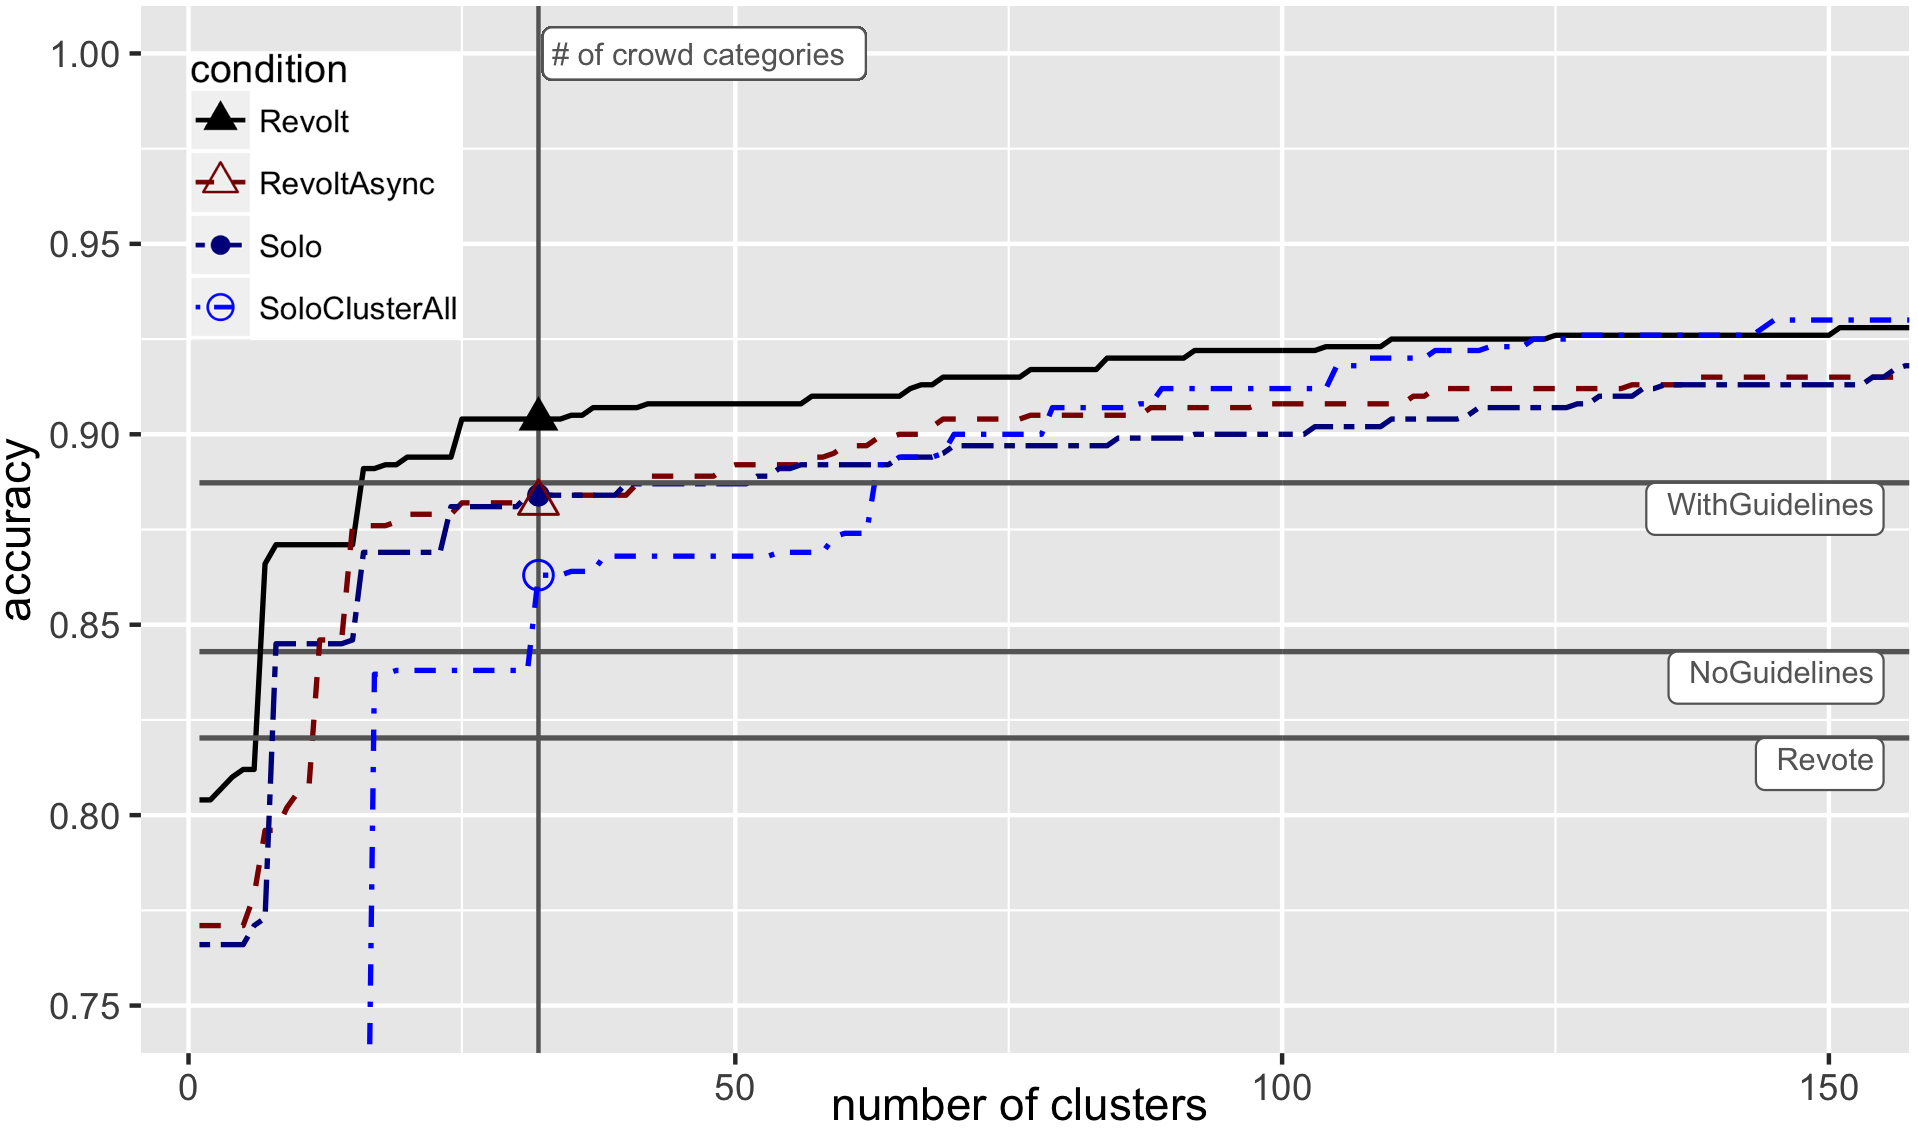
\includegraphics[width=0.7\columnwidth]{Chapters/Revolt/figures/curveR2.png}
	\caption[Accuracy of different approaches as a function of post-hoc requester effort.]{
	Accuracy of different approaches as a function of post-hoc requester effort (i.e., number of clusters) for the Car1 dataset. 
	}
	\label{fig:curve}
\end{figure}


In addition to presenting crowd-generated categories, Revolt (and its variant conditions) can also algorithmically produce clusters of uncertain items at various levels of granularity for requesters to review (see the Revolt Section). As a result, requesters can vary the amount of effort they are willing to provide to produce final label decision boundaries in these conditions. Therefore, for these conditions, we also report on accuracy achieved at various levels of post-hoc requester effort. As an example, Figure~\ref{fig:curve} shows how the accuracy of Revolt changes for different amounts of requester effort required to assign labels (estimated by number of clusters needing labels) on the \emph{Car1} dataset. For this example, receiving requester input for 32 categories produced by Revolt (see vertical line in Figure~\ref{fig:curve}) achieved an accuracy higher than the upper bound WithGuidelines baseline, while other conditions did not. 

We compare the accuracies of different conditions in two ways. In Table~\ref{tab:accuracy}, we compare conditions at a fixed amount of post-hoc requester effort (i.e., the number of clusters needing examination by the requester). We fix effort to be the number of categories generated by the crowd under the Revolt condition for each dataset. For example, for the \emph{Cars1} dataset, we compute accuracy at the point where 32 clusters would need to be examined. The accuracy results presented in the \emph{Cars1} row in Table~\ref{tab:accuracy} therefore corresponds to a vertical cut of Figure~\ref{fig:curve} at the 32 number of clusters mark. To compare different conditions and baselines, we fit one generalized linear model per baseline, predicting correctness as a function of condition, with dataset as an additional factor to account for item variation. Both models significantly improve fit over a simpler model with dataset
as the only variable (X2(5)=160.1, $p<0.01$, and X2(5)=180.9,
$p<0.01$). 
Using the models, we ran general linear hypothesis tests for pairwise comparisons between conditions, and used Tukey's honestly significant difference as the test statistic. 
The models showed both Revolt and RevoltAsync to be significantly more accurate than the lower bound NoGuidelines condition (B=0.56 and 0.38, both $p<0.01$) while no significant differences were found when comparing to the upper bound WithGuidelines condition (B=0.05 and -0.13, p=0.99 and 0.63).


In addition to using a fixed numbers of clusters, Figure~\ref{fig:accuracy} shows the of accuracy improvement rate of each condition under different levels of requester effort relative to the NoGuidelines baseline. Since the smaller datasets only had less than 30 uncertain items, for conditions that generate rich structures (Revolt, RevoltAsync, Solo, and SoloClusterAll) we show the accuracy improvement rate for 10, 15, 20, and 25 post-hoc judgments for the smaller webpage datasets, and 10, 20, 30 for the larger image datasets. We also report the accuracy improvement for the WithGuidelines and Revote conditions that do not require post-hoc judgments. 





%\saleema{Needs work. State the goal (need to measure cost), then the problem (couldn't compare because of different implementations, then solution (estimating one with the other)}

%Revolt produces reusable structures that generates accurate training labels without the efforts of guidelines creation. However, one critical question is the cost of such system comparing to traditional approach and the different conditions. 
In our experiments, \$3 were paid to each worker for participating in a batch of Revolt, Revote, Solo, SoloClusterAll conditions, where \$1 was paid as base payment for completing the first stage, and \$2 bonuses were added for completing the rest of the stages. For the RevoltAsync condition, \$1 was paid for each Vote and Explain task. We adjusted the number of items in each batch so that crowdworkers could finish batches under 20 minutes including time spent waiting for other crowdworkers. Each batch in the image datasets contained around 60 items while each batch in the webpage datasets contained around 27 items. For the baseline conditions, we paid \$0.05 for labeling one image, and \$0.15 for labeling one webpage. 

We also compared cost of each condition in terms of crowdworker work duration (Figure~\ref{fig:runtime}). For our Revolt, Revote, Solo and SoloClusterAll, we measure work duration directly by tracking crowdworker behaviors using our external HIT interface, tracking mouse movements to identify the exact time crowdworkers started working after accepting the HIT. Our NoGuidelines, WithGuidelines, and RevoltAsync conditions were implemented via the Mechanical Turk form builder feature. While Mechanical Turk does report work duration, crowdworkers often do not start work immediately after accepting a HIT. To correct for this, we approximate the work duration for these interfaces in the following way. We approximate the work time of the NoGuidelines and WithGuidelines conditions (our baseline conditions) using the timing statistics collected from the Vote Stage of the Revolt workflow, as the crowdwork involved in these baselines are of the same nature as the Vote stage. We similarly approximate the total work duration for the RevoltAsync condition by using the timestamps from the Solo condition (where crowdworkers provided explanations for each item), and multiplying the average duration with the number of uncertain items identified for each dataset in this condition.
 




%\ece{Do we want to discuss the reusability of the data anywhere? Do we collect data for two versions of the data set separately or collect the data once and then customize it for each data set using requester input? If it is the second one, it is a good argument for reusability of labels and we should emphasize that. }


%\saleema{Joseph, this section needs work. 1) You're mixing Results with Discussion. Typically Results are just where you present raw data and any stats you may have. Then in the Discussion you discuss your interpretations of the results. You can either try to separate the two or keep it, but then you have to figure out what to do with the current Discussion. 2) The subsections are not clear. First, avoid subsubsections where possible. If you want to keep Results mixed with Discussion, you shoudl just have a bunch of subsections such as: "Revolt vs Traditional Labeling", "Forcing Crowdworkers to Choose", "Benefits of Real-time Collaboration". For each of these you can mix the accuracy and cost results and discussion.  3) I'm worried about the Cost Analysis section. In particular, the formulas in Table 4 are cool in theory but without estimates for each T* I think you might be opening yourself up to reviewer criticism. Its not really that helpful wihtout the estimates anyways. It also makes the worktime per item analysis weird because its clear from the formulas that in most cases wortime is not uniform across N. You might want to consider removing this and just talk about the monetary cost (when will that be in??) and worktime per item in each of the subsections if you end up mixing accuracy and cost.}

\begin{figure}[ht]
	\centering
	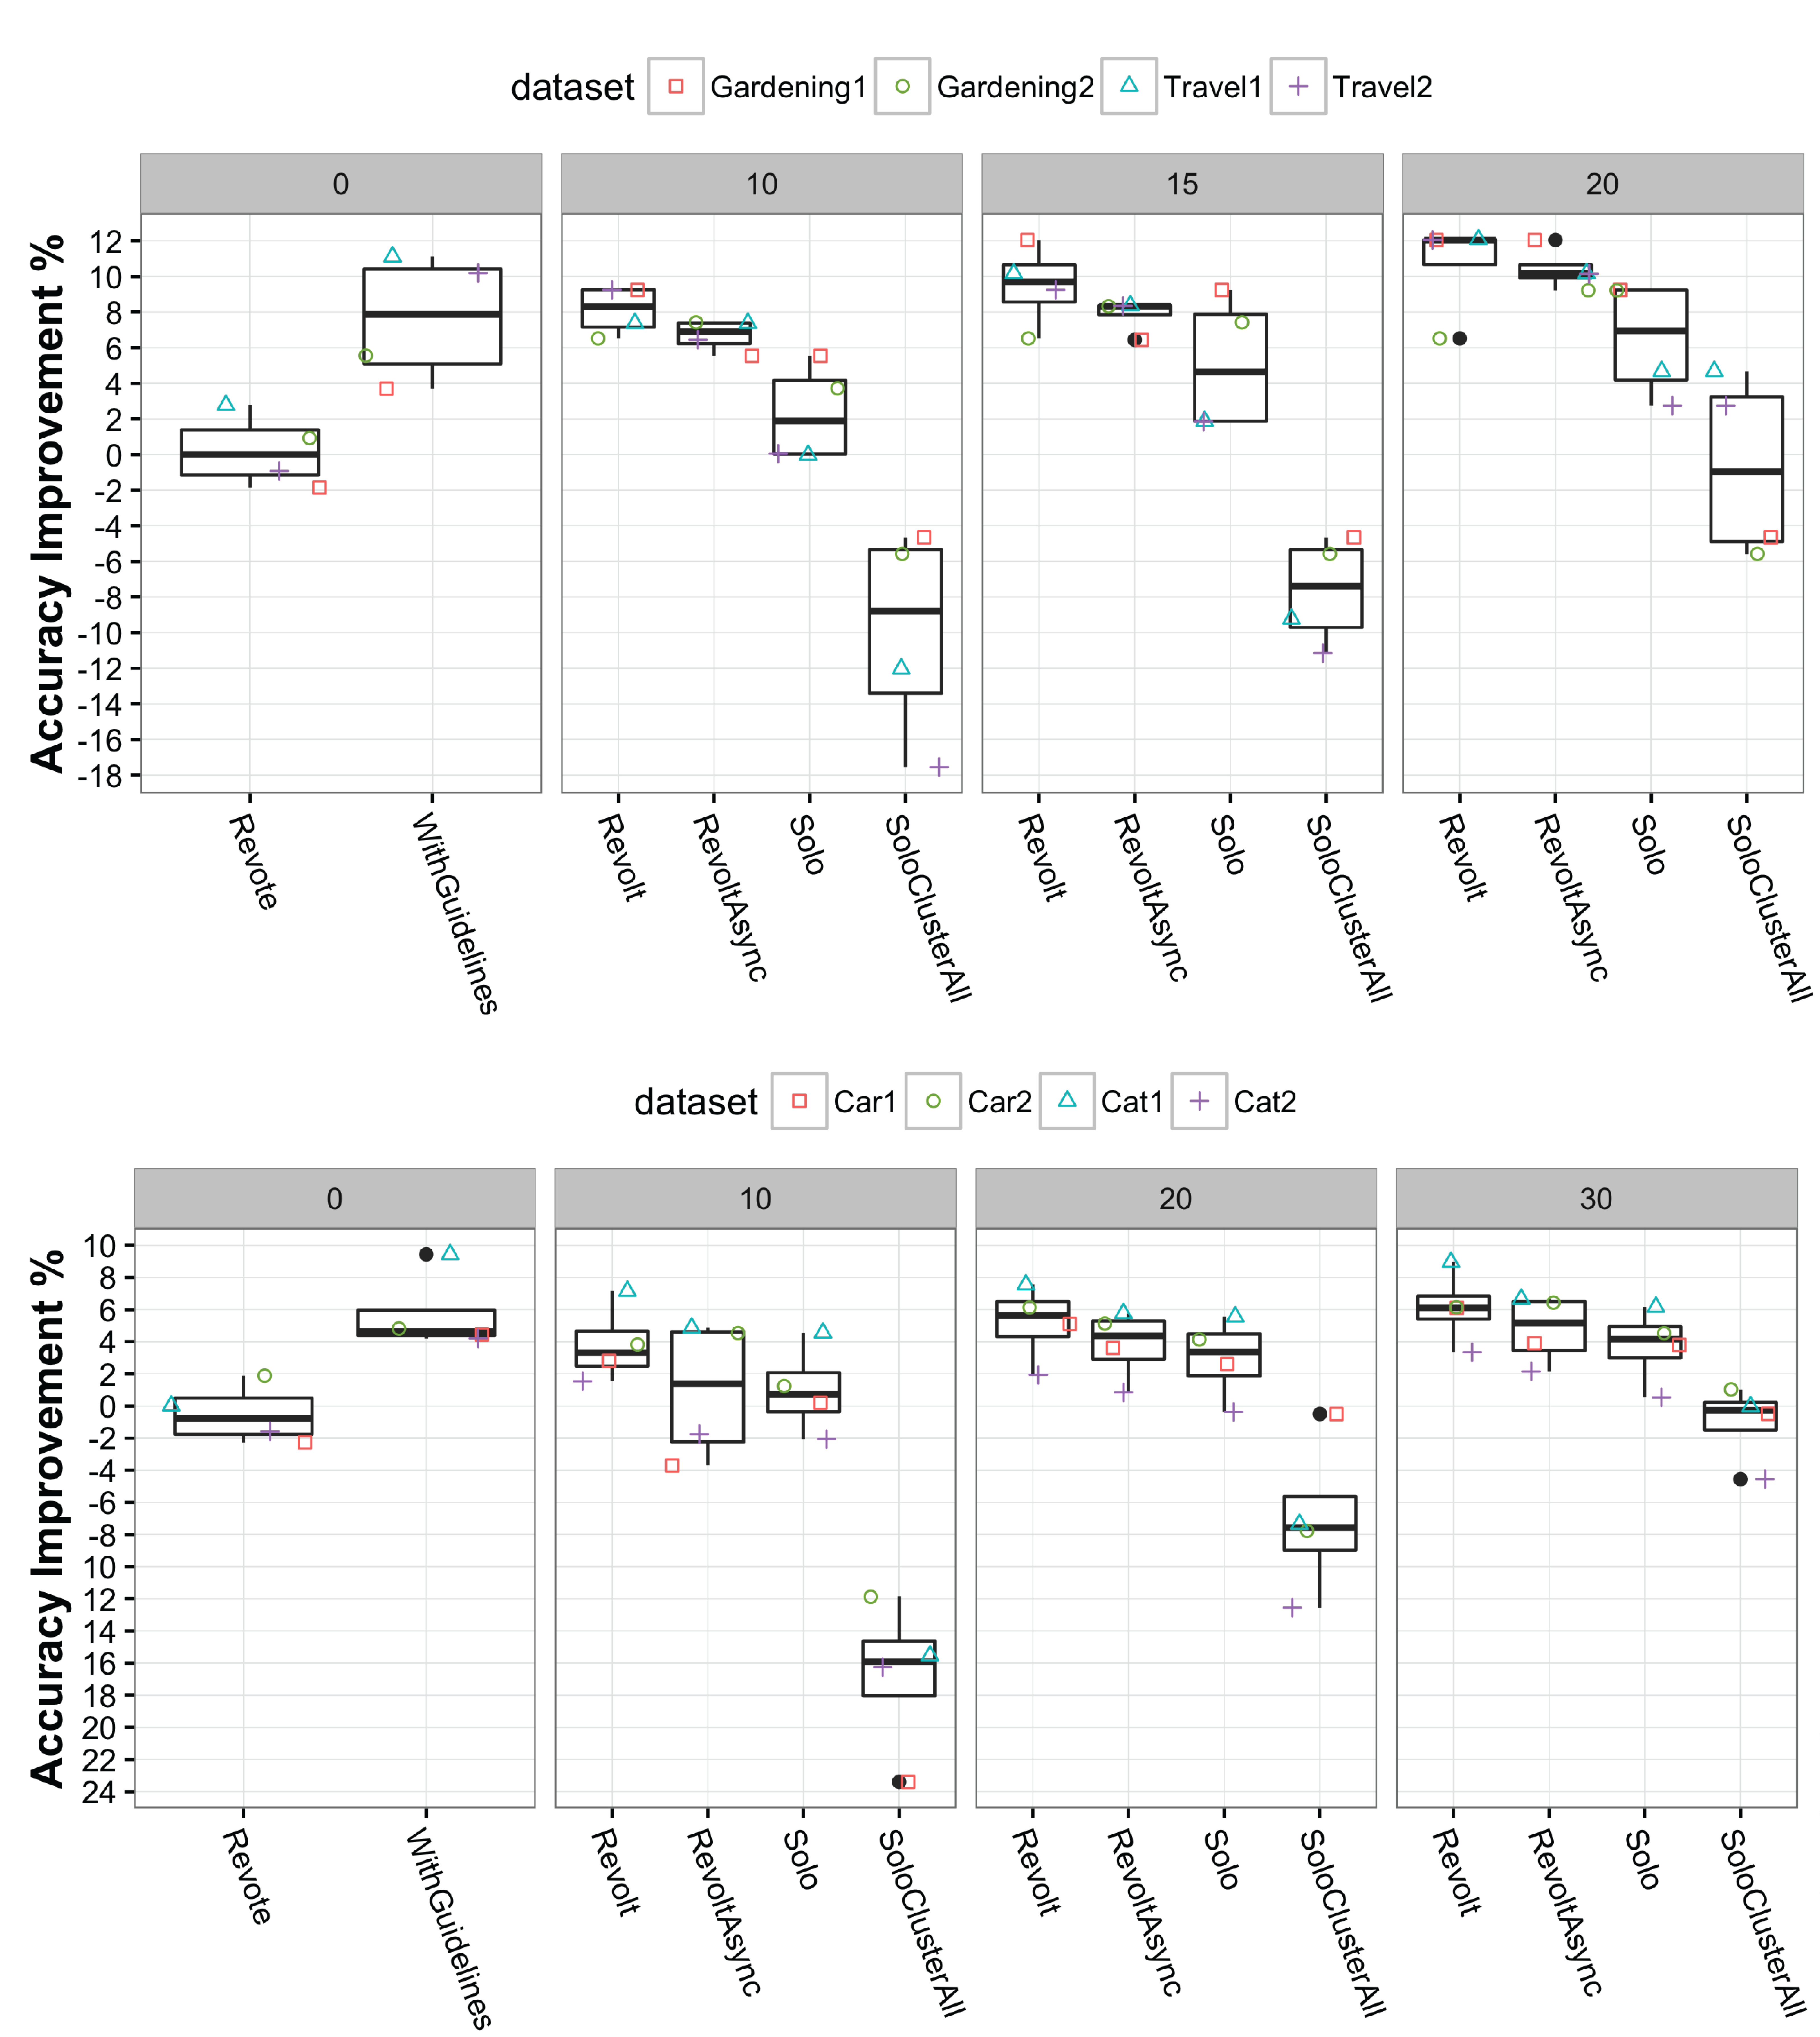
\includegraphics[width=0.7\columnwidth]{Chapters/Revolt/figures/haccuracy2.png}
	\caption[
	Accuracy improvement as a function of requester effort. 
	]{
	Accuracy improvement of different conditions over the NoGuidelines baseline as a function of requester effort. 
	}
	\label{fig:accuracy}
\end{figure}


%\subsection{Labeling Accuracy}

\subsubsection{Revolt vs Traditional Crowdsourced Labeling} 

%\saleema{NoGuidelines is not really a realistic scenario. I would go back to the conditions, explain that NoGuidelines should be considered a lower bound since in most traditional uses of crowdsourcing, some guidelines are provided. That way NoGuidelines is presented as a lower bound and WithGuidelines is an upper bound. Then revise this section accordingly  and say that the real traditional crowdsourcing falls somewhere in between. Nevertheless we can see that Revolt performs etc....}

In both traditional crowd-based labeling and Revolt, requesters examine uncertain items to refine the label boundaries. However, in Revolt, this is done at the category level in a post-processing step as opposed to reviewing items, refining instructions, and launching more tasks in a loop. The latter may lead to wasted work, particularly when refinements require workers to relabel the same items. In Revolt, structures captured from crowdworkers during labeling allow requestors to refine label boundaries post-hoc without having to launch more tasks.

When compared against the NoGuidelines condition (the lower bound of traditional crowdsourced labeling), Revolt was able to produce higher accuracy labels across all eight datasets (Table~\ref{tab:accuracy}). 
The generalized linear models also showed both Revolt and RevoltAsync to be significantly more accurate than the NoGuidelines condition.
The comparison of the NoGuidelines and WithGuidelines conditions shows that comprehensive guidelines indeed increase labeling accuracy across all eight datasets (Figure~\ref{fig:accuracy}), but at the cost of the effort needed to create comprehensive guidelines in advance. 
%This result supports the assumption that task uncertainty can also be an important factor for low quality results in crowdsourcing. \saleema{This last sentence comes out of nowhere and doesn't explain how it imapcts anything. Expand on this perhaps in its own section or at least in its own paragraph.}
In contrast, Revolt was able to produce comparable accuracy without any guidelines. In fact, in 6 out of the 8 datasets we tested, Revolt was able to produce labeling accuracies slightly higher than the upper bound baseline 
(Table~\ref{tab:accuracy}). The generalized linear models also showed that neither Revolt nor RevoltAsync were significantly different than the upper bound condition (B=0.05 and -0.13, p=0.99 and 0.63).
This suggests that Revolt can outperform current best practices for crowdsourcing training labels where guidelines provided by the requesters are likely to be less comprehensive than the ones provided in the WithGuidelines condition. That is, Revolt shows promise to improve the quality of labeled data collection while removing the burden of comprehensive guideline generation by making use of collaborative crowdsourcing approaches.


%\subsection{Reusing the Rich Structures}

%\saleema{Here you can also add a bit about reusability as Ece suggested. You can even present your results on using different guidelines for the same results to show reusabiliyt. Then you can explain that Traditional doesn't transfer to diffrent guidelines. You could even add a subsection about it called Reusability of Revolt Results.}


\begin{figure}[ht]
	\centering
	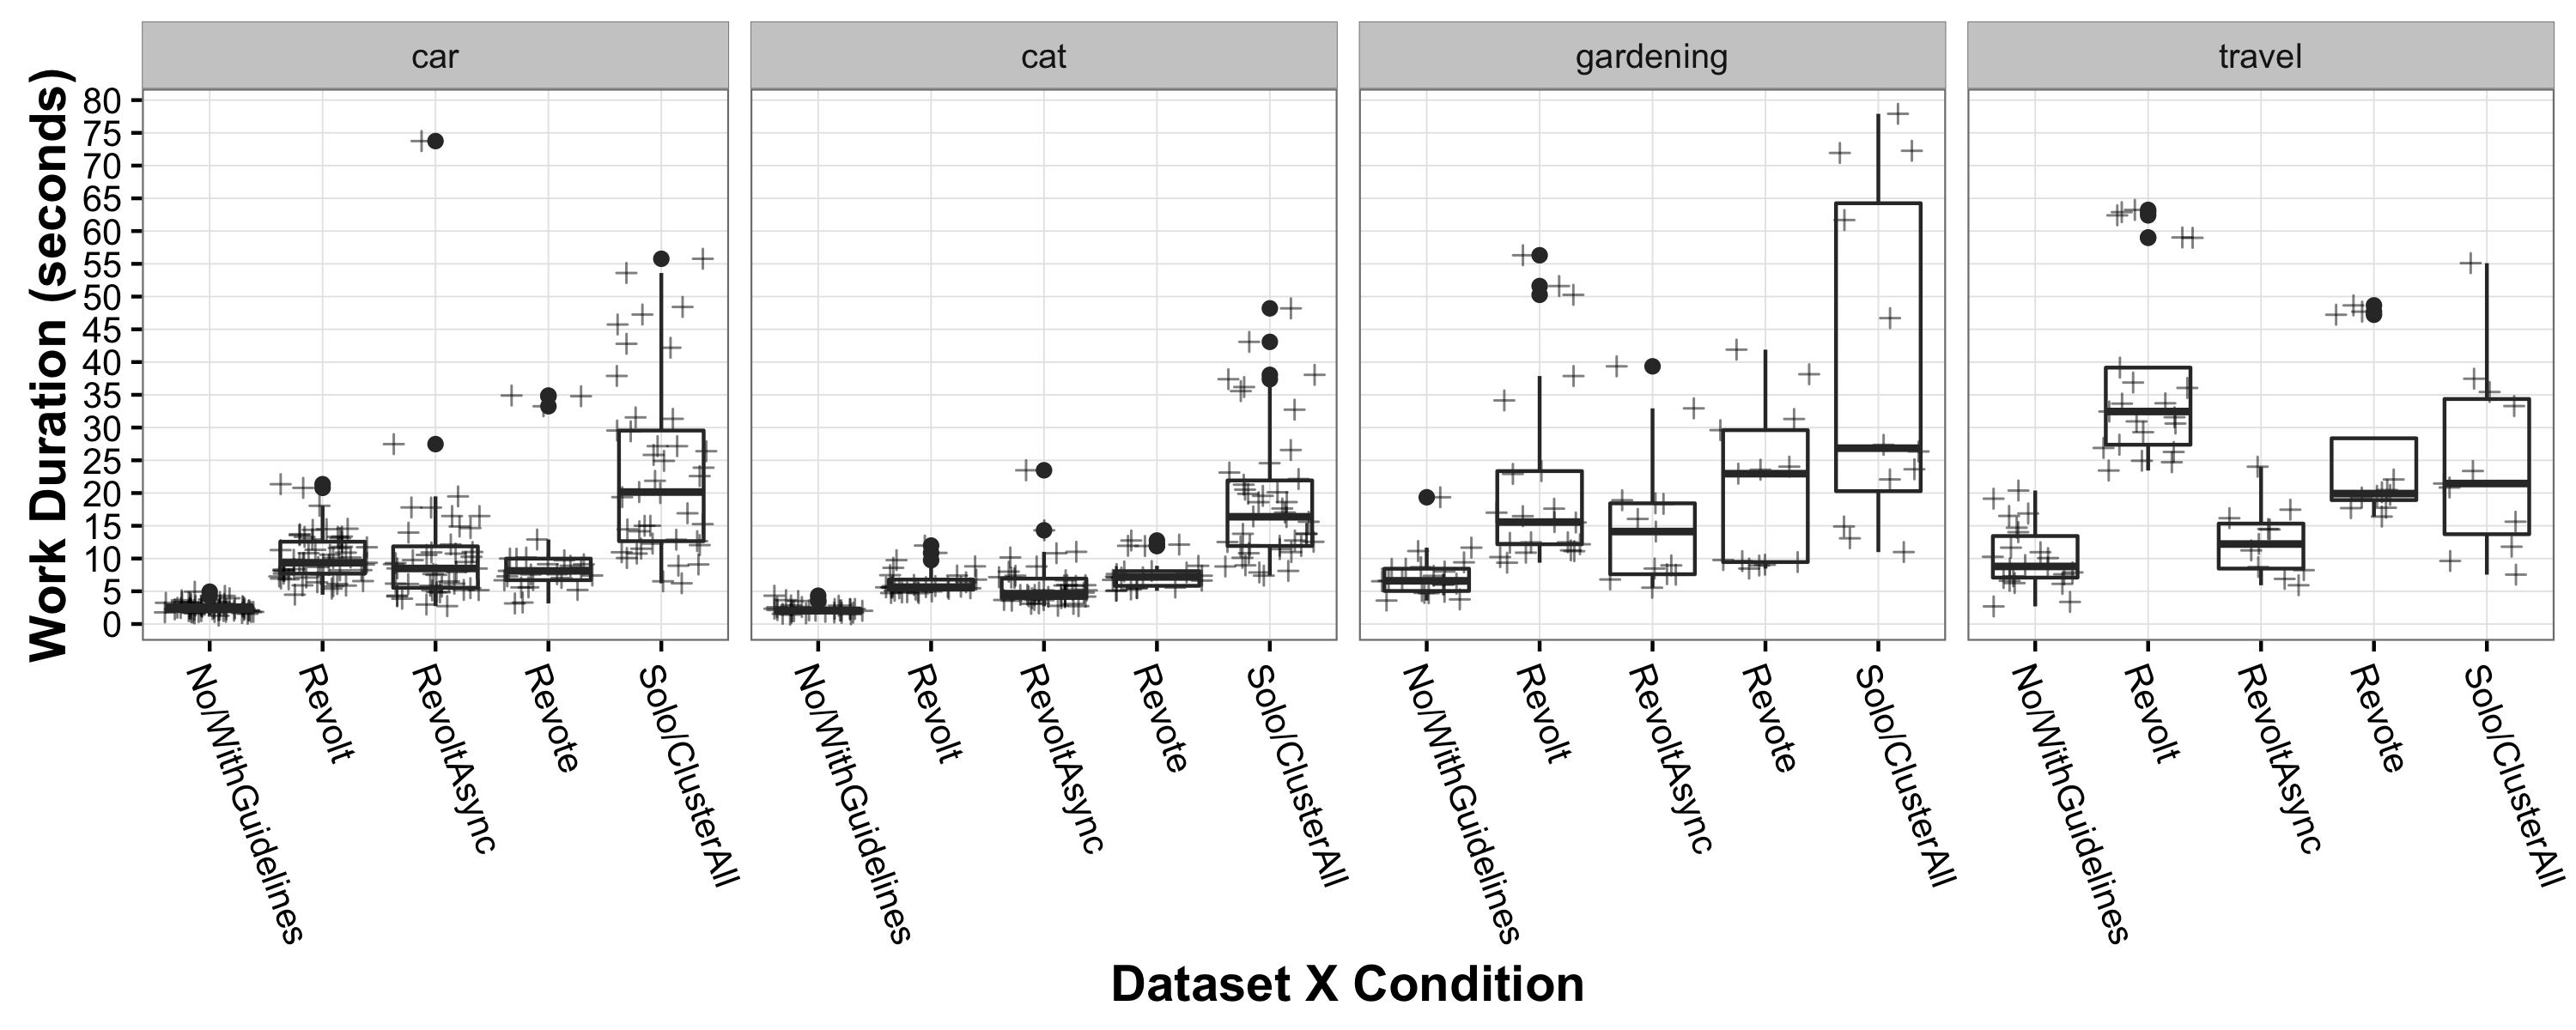
\includegraphics[width=1\columnwidth]{Chapters/Revolt/figures/runtime.png}
	\caption[
	Work duration of each crowdworker under different conditions. 
	]{
	Work duration of each crowdworker under different conditions, normalized by the number of item in each batch. 
	}
	\label{fig:runtime}
\end{figure}


\subsubsection{Forcing Crowdworkers to Revote} 

An alternative way of explaining why we see uncertain items with conflicting labels in Revolt's Vote Stage is that crowdworkers could converge on true concepts for all items but they are simply making mistakes while labeling. To test this, the Revote condition allowed crowdworkers to reconsider their labels after seeing explanations from others, providing the opportunity to correct mistakes.
While previous work has shown accuracy improvement using this strategy under a scenario where clear guidelines were given to pre-trained crowdworkers \cite{drapeau2016microtalk},  
%\saleema{I'd reverse the following two sentences. State your result and then state that this is a contradition to previous work and then explain what your hypothesis is about it}
results from our study showed that the Revote condition did not improve labeling accuracy compared to the NoGuidelines lower bound baseline (B=0.03, p>0.99), with near zero median accuracy improvement (Figure~\ref{fig:accuracy}).  This suggest that in scenarios where it is infeasible to generate comprehensive guidelines to guide workers towards a single correct answer, accuracy cannot simply be improved by quality control on individual workers; instead allowing crowdworkers to inform the requesters about their confusions and discoveries may be a better strategy than forcing them to make arbitrary decisions and then performing post-hoc quality control.
%\saleema{So in the previous work where accuracy was improved, did they assume a single correct label? If so, then are you disproving their result? Or did they do something slightly different. You have to be careful aobut the distinctions you make here.}

\subsubsection{Benefits of Collaborative Crowdsourcing}

Traditionally, crowdsourcing techniques require independent crowdworker judgments and do not permit knowledge sharing. 
In this work, we investigated the benefits of collaborative crowdsourcing by allowing limited and structured communications between crowdworkers. Our collaborative conditions (Revolt, RevoltAsync, Revote) presented crowdworkers with different combinations of conflicting judgements, justifications for the conflicting judgements, and proposed structures (i.e., category names) from other crowdworkers, either synchronously or asynchronously. On the other hand, in NoGuidelines, WithGuidelines, Solo, and SoloClusterAll conditions, workers were not presented with any judgments from others.

%\ece{Isn't it the case the Revolt sync does better in many conditions? Then we should say that instead of saying comparable. Because if accuracies are comparable, it makes no sense to use Revolt instead of Revolt async. It is important to highlight the trade-off between accuracy and time if it exists.  }
%\saleema{The improvements are very small and without stats to show that its better its a stretch to argue for Revolt over RevoltAsync. I'd be okay with us saying "slightly better" or something.}
Comparing Revolt to RevoltAsync, Revolt with synchronous stages performed slightly better than RevoltAsync at the cost of slightly higher worktime (Figure~\ref{fig:runtime}), but the difference was not significant (B=0.18, p=0.28). Comparing collaborative and non-collaborative conditions, results show that both Revolt and RevoltAsync outperformed the non-collaborative Solo condition for each  dataset we tested (Figure~\ref{fig:accuracy}). Based on the generalized linear models, the real-time collaborative Revolt condition achieved significantly higher accuracies than the  
non-collaborative Solo condition, while the RevoltAsync variant did not (B=0.24 and 0.06, p=0.04 and 0.97). 

Interestingly, we initially expected the RevoltAsync condition would yield poorer results compared to the non-collaborative Solo condition due to cognitive dissonance (i.e., asking one crowdworker to explain the label of another). However, the results showed no significant difference between the two conditions. On the other hand, the non-collaborative SoloClusterAll condition, where explanations were collected for all items to cluster both certain and uncertain items, performed worse than the lower bound baseline. These results suggest that identifying and presenting disagreements is an important factor for eliciting meaningful explanations, even when the disagreements were presented to different crowdworkers in an asynchronous setting (Figure~\ref{fig:accuracy}). 

%To investigate the benefits of real-time collaborative crowdsourcing, we also compared Revolt to variants that removed the real-time and collaborative components (RevoltAsync, Solo, SoloClusterAll). Results suggest Revolt outperformed its non-collaborative variants when having the same amount of post-hoc requester effort (Figure~\ref{fig:accuracy}), suggesting real-time collaboration might be a key factor contributing Revolt's accuracy improvement. Comparing the three non-collaborative conditions, the SoloClusterAll condition that clustered both certain and uncertain items performed the worst. This suggest identifying certain and uncertain regions of the data is an important component of Revolt, and clustering all items in attempts to correct the unanimously voted errors may not be an effective strategy. \saleema{This is not an explanation. This is just a result. Give a hypotheses as to why you think clustering all the data didn't work. Perhaps look at your clustering results to give examples of where this might break down.}



%\begin{figure*}[!ht]
%	\centering
%	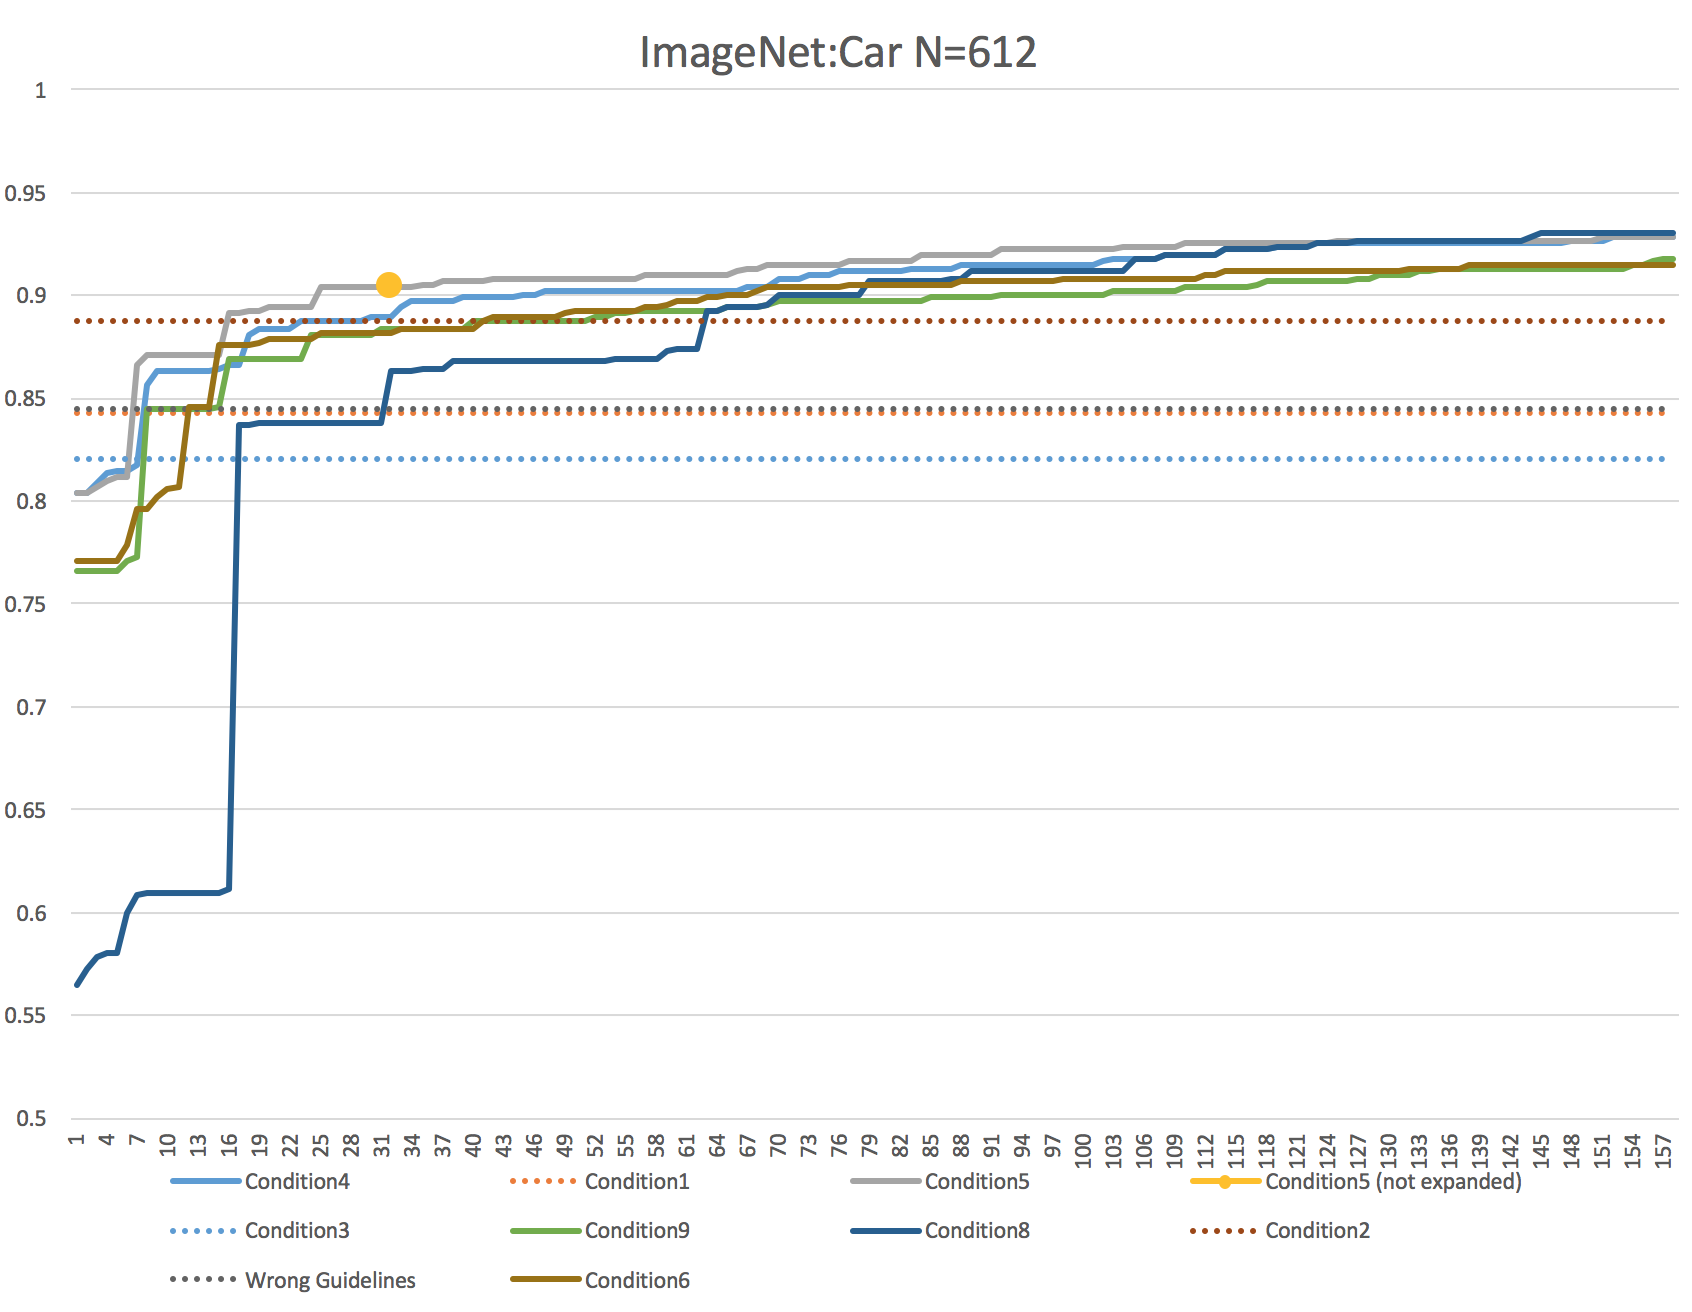
\includegraphics[width=1.0\columnwidth]{figures/dataset1.png}
%	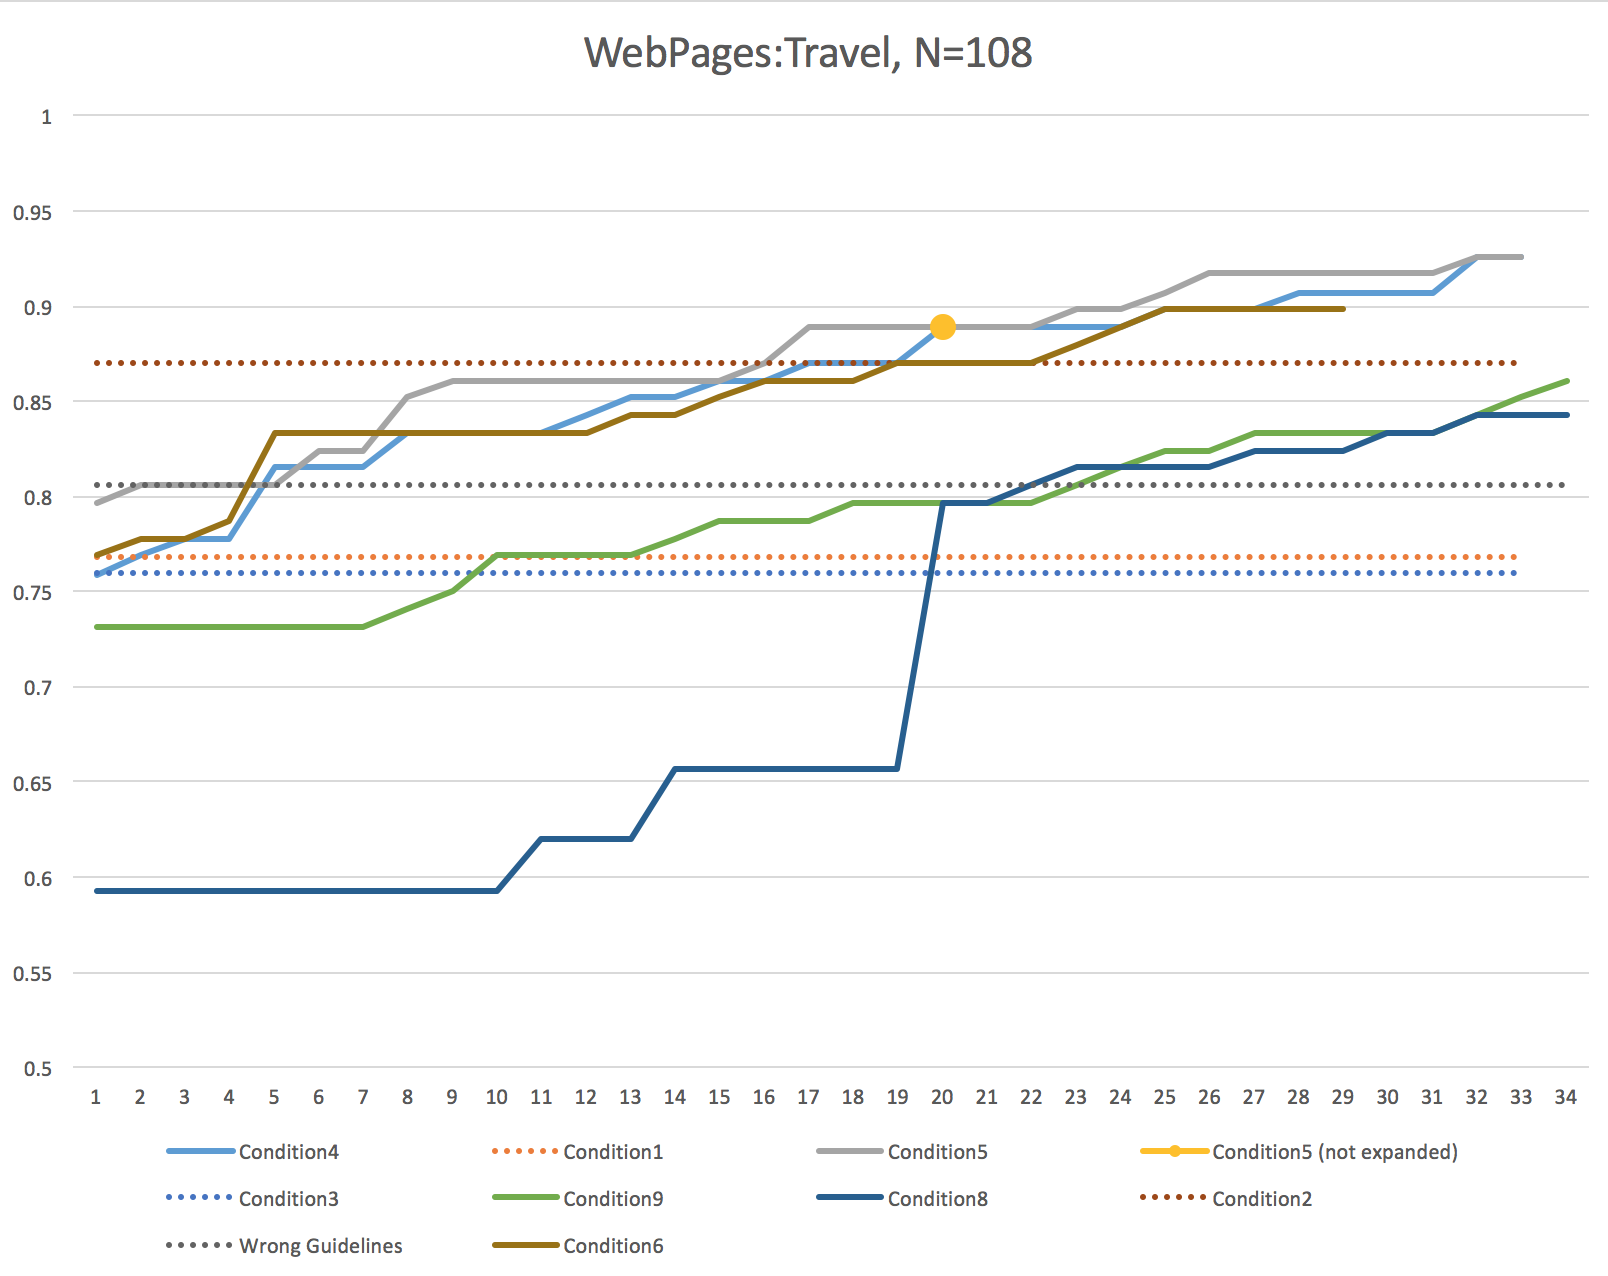
\includegraphics[width=1.0\columnwidth]{figures/dataset2.png}
%	\caption{
%	}
%	\label{fig:accuracy_curve}
%\end{figure*}




\subsubsection{Cost Analysis}


In general, items in the webpage datasets took longer to label compared to items in the image datasets. This is to be expected since webpages typically contain both text and images and therefore often require more effort to comprehend (Figure~\ref{fig:runtime}). 
Comparing different conditions, traditional labeling (WithGuidelines, NoGuidelines) that only required crowdworkers to label each item had the lowest work times, and the real-time collaborative conditions, Revote and Revolt, had similar and higher work times. This suggests categorizing or re-labeling items has similar costs, but creating rich structures for post-hoc requester judgments can lead to better accuracies. The RevoltAsync condition showed lower work time compared to the Revolt condition. This is also to be expected since crowdworkers did not need to wait for others during the task for progress synchronization. The non-collaborative workflow conditions Solo and SoloClusterAll has the highest work time since it required explanation of all certain and uncertain items. Therefore, using the voting stage to identify uncertain items and guide efforts on structure generation can improve accuracy while also lowering cost.

One concern for synchronous collaborative crowdsourcing is crowdworkers idling or returning the HIT before the task is competed. This was especially important since we did not include a method for using labels from groups with missing labels. In sessions with drop-outs, we paid the crowdworkers and discarded their labels. In fact, the first prototype of Revolt had a high dropout rate of around 50\% (i.e., half of the crowdworkers did not complete the three stages), making it infeasible for practical use. Through an iterative task design process, we observed the following mechanisms being effective for reducing drop-outs: Explaining the collaborative nature of the task, providing time estimates in the task instructions, adding example items in the preview screen so crowdworkers knew what to expect if they accepted the HIT, sending desktop and audio notifications to help coordinate workers, and giving clear progress indicators throughout the tasks (e.g., current bonus amount, number of remaining stages, and the amount of bonus for completing each stage). In the final version of the task with these mechanisms, the dropout rate was lowered to an average of around 5\% for the eight datasets presented in this chapter.

\section{Discussion}

%We compared our conditions using datasets of variety formats (images, webpages) and size (around 100 and 600 items). We used \emph{cars}, \emph{cats}, \emph{travel}, and \emph{gardening} to show that uncertainty can exist in crowdsourcing labeling tasks even for seemingly simple and generally familiar concepts (Table~\ref{tab:accuracy}). \saleema{In the discussion, reiterate this point and say that we show differences even for seemingly simple concpets. we would expect the differences to become even more pronounce for mor complicated concepts}

%\saleema{Much of this paragraph will be redundent if you merge the discussions from the previous section with this.}We tested Revolt against 6 baselines and variant conditions using 8 gold-standard datasets with up to 600 items consisting two different formats (webpages and images).
%Experimental results suggest that Revolt can to produce high quality labels without the need for the requesters to engage in the difficult task of guidelines creation. The real-time and collaborative nature is also beneficial as evidenced by comparing Revolt to its asynchronized variants.

%\joseph{note: testing different redundancy} 

%\joseph{note: matching worker with the same skill level to avoid waiting time.} 

%\saleema{I think these first two paragraphs are eithr not relevant or out of place given the reframing. Can you add any comments about general limitations of Revolt plus Revolt Async? Or if you think Revolt still could have benefits for some reason, argue for why. Otherwise, just change this section title to Future Work}

%\saleema{This is too specific to one stage of Revolt and given that it might not be necessary, since RevoltAsync doesn't have it, why do we care? If you want to talk about this, relate it back to why you think Revolt is better than RevoltAsync}One obvious limitation is the strong ordering effect of Revolt's real-time categorization mechanisms. For example, if the category \emph{big cats} was created early in the process, Revolt might lose its hyponymous concepts such as \emph{lions} or \emph{leopards}, and the requesters would need to rely on the automatic clustering process to recover these concepts based on the explanations. Revolt also made the assumption that crowdworkers will be able to select the best category, which can potentially be challenging as the list of categories grow in length. Even when the assumption holds true, better categories could be added even after a crowdworker completed the task. Adapting previous crowd clustering approaches to  real-time settings or developing more sophisticated real-time crowd clustering methods are fruitful areas of future work.

 
%\saleema{This doesn't seem relevant anymore since the RevoltAsync condition doesn't require wiating and should be able to handle different reading speeds. I'd cut}Another limitation is when the items are difficult to comprehend by the crowdworkers. We encountered this limitation when trying to run Revolt on a dataset of legal and financial news, where crowdworkers were tasked to determine if the main theme of an article is about ``\emph{an legal issue for an organization}''. We found that the crowdworkers were reading items in this dataset at very different speed in each stage, making it difficult to estimate the right number of items per batch to avoid long waiting time. Ultimately, the inherent difficulty the dataset lead to high dropout rate, and Revolt was unable to finish labeling all items.

%\saleema{This is confusing. Your basically saying thta Revolt can't handle overly complex topics. Itsn't that the whole idea? What is a manageable set of catgories? How many wree produced here and is that more than the other cateogires? I would cut this unless you want to do a deep analyais. I think the problem is just the first part which is the different labeling speeds which increases wait time and therefore drop out rates. This is not something encountered in non-realtime systems. Give some ideas to counter this in future work such as perhaps estimating reading speeds of crowdworkers to match up skill level/reading speed levels to avoid dropouts. }
 


%\saleema{Restate main findings and takeaways. Revolt produces high quality labels without the need for guidelines. The real-time nature is helping as evidenced by our async results. Areas for improvement in the system E.g., stemming of category tags for better grouping, cleaning up labels post-hoc (some workers said they made mistakes in labeling). }

%\saleema{In the discussion section, be sure to talk about the limitations of our current technique (e.g., that the categorization is highly impacted by the order in which items and categories appear) and some of the other options we discussed about trying to improve this more (e.g., to get people to categorize at the right level). Use examples of poor categories from your results to seed this discussion. }

%\saleema{Discuss anything about the impact of dataset size or difficulty. You could mention the legal dataset here}

In this work we focused on designing Revolt's collaborative crowdsourcing workflow and evaluating whether the generated structures contain information with enough richness for label requesters to define accurate label decision boundaries. 
While we believe the proposed mechanisms of identifying uncertainty with disagreements and creating structures with explanations can generalize to multi-class scenarios, the added complexity to both the crowdworkers and the interfaces should be studied further. Research is also needed to design a requester-facing interface depicting these structures and to compare requester effort in post-hoc analysis with guideline creation. 

%\ece{what was the pain point you were trying to address if they already had guidelines? Are you testing how good their guidelines were?}
To gain insights into these future directions, we conducted a small follow up experiment where we ran Revolt on data needed by a group of practitioners from a large technology company for a real machine learning research problem. 
This group required 300 items from the publicly available 20 Newsgroup Dataset \cite{Newsgroups20} to be labeled as being about ``Autos'' or ``Not Autos''.
Prior to our study, the group of three practitioners already spent approximately 2-3 hours each to browse through some of the data and then about 1-2 hours to generate and iterate over the guidelines. This is a typical process for guidelines creation analogous to previous work  \cite{wiebe1999development}, and should represent a realistic scenario somewhere between our lower bound NoGuidelines and upper bound WithGuidelines conditions. Because the practitioners already had some idea of how they wanted the dataset labeled, we ran Revolt with their guidelines. %\saleema{Joseph I reverted this. We don't want to say that this is a more realistic scenario. You cut out the bit later on about how the guidelines were actually harmful. But I think the fact that we still surfaced a bunch of new categories given the guidelines shows that this can be useful even with guidelines. You could add a line about that if you think its necessary.} 
%(e.g., "buying, owning, driving, maintaining and/or understanding cars is about autos", "mentioning autos as setting, background material, or comparison in a discussion that is clearly focused on another topic should not be considered as about autos").
%Because the group already had some ideas about how they wanted the data to be labeled as a result of the guideline creation process, we ran Revolt with their guidelines in the instructions. 

We presented Revolt's results to one member of the research group and asked them to examine the resulting structures. Interestingly, 93 out of the 300 items (31\%) were inconsistent even though we gave crowdworkers guidelines about how to label, underscoring the difficulty of creating comprehensive guidelines covering the subtleties in a dataset. These items surfaced 23 unique categories and, to the practitioner's surprise, 70\% were not covered in the original guidelines (e.g., auto accessories, insurance, intoxication). 7 of the categories were mentioned in the guidelines with explicit instructions about how to label (e.g., driving, buying/selling, auto repair), indicating either failure of some workers to learn the guidelines or failure of the guidelines to capture the complexity of these categories. 
For example, one of the items categorized as driving was about which side of the road people should drive on. While this could be considered about auto driving, it could also be about driving other types of vehicles. %Worker explanations about this item surfaced this ambiguity: \textit{"While it was related to driving it wasn't related to Auto in itself. For instance, motorcycles could also be considered in this conversation."}, \textit{"This is talking about what side of the road people drive on and relating to car exports."}, and \textit{"I didn't think this one was pertaining to autos specifically, just roads in different countries."}
%For example, one of the items categorized as driving was about which side of the road people should drive on. While this could be considered about auto driving, it could also be about driving other types of vehicles. Worker explanations about this item surfaced this ambiguity: \textit{"While it was related to driving it wasn't related to Auto in itself. For instance, motorcycles could also be considered in this conversation."}, \textit{"This is talking about what side of the road people drive on and relating to car exports."}, and \textit{"I didn't think this one was pertaining to autos specifically, just roads in different countries."}
Reading crowdworker explanations helped the practitioner to better understand this ambiguity, and led them to second guess their original guideline about labeling driving related items as autos.  The practitioner we interviewed also suggested additional ways they wanted to use Revolt's results, such as removing ambiguous items or certain categories before training a model, or creating features around categories that surfaced. Further research is necessary to examine the potential for Revolt's rich structures to support these tasks.
%Importantly, while the practitioner would be able to reassign items Revolt flagged as driving to the "not auto" category, Revolt may have still assigned some driving related items to the "auto" category because they were in the guidelines. That is, reassignment in this case could lead to inconsistent labels and poor machine learning. One possible alternative technique for incorporating guidelines into Revolt when they are available could be to seed the list of categories visible to crowdworkers during Revolt's categorization phase to help them tag items according to the requester's desired instructions.

The practitioner also made several suggestions with respect to how one might design the presentation of Revolt's structures. First, an indicator of category quality or confidence based on the distribution of labels assigned by individual workers would have helped the practitioner prioritize which categories to look at first and how much to examine each category before making a decision (e.g., by reading individual explanations or viewing a few of the individual items within a category). Other suggestions included blacklisting certain items from the category list (e.g., ``autos'' surfaced as a category), presenting structures within hierarchical categories, and searching explanations for to find related items under different categories. Future research should consider these insights in determining how to efficiently present Revolt's structures to label requesters.


%\section{Conclusions}

%In this paper, we explored an alternative process of crowdsourcing training labels for machine learning by forming small, ad-hoc teams on crowdsourcing markets and allowing crowdworkers to engage in collaborative exploration of the uncertainty in datasets by exchanging prospectives using a synchronized three stage workflow. 

In this chapter, we presented Revolt, a new approach for generating labeled datasets for machine learning via collaborative crowdsourcing. Our experimental results comparing Revolt to traditional crowd labeling techniques demonstrates Revolt can shift the efforts of label requesters from a priori label guideline creation to post-hoc analysis of crowd-generated conceptual structures. This has several benefits including potentially surfacing new or ambiguous concepts unanticipated by label requesters, reducing the amount of crowdworker training and effort required to learn label guidelines, and allowing label requesters to change their minds about label decision boundaries without having to re-collect new data. 

%\section{Acknowledgments}

%The authors would like to thank Andrew Mao and Walter S. Lasecki for the insightful discussions, and Joel Chan for the assistance in analyzing the evaluation results.

%%% Local Variables:
%%% mode: latex
%%% TeX-master: t
%%% End:
